\chapter{Optical Network Interface Design} % Write in your own chapter title
\label{ResultsSS}
%\addtotoc{State of the Arts}
\lhead{\emph{Experimental Results on SmartSense}} % Write in your own chapter title to set the page header
%\section{Experimental Results}
\section{Introduction}
In the context of this thesis, the sensor signal processing to extract the state of devices is not studied nor implemented. We just focus on how to transform this information to probability feature to help the existing NILM algorithms to improve their performance. Therefore, with each dataset applied to the simulation in Matlab, we assume a WSN monitoring some specific devices. The operation of these devices can be detected with a certain accuracy.
To evaluate the WSN performance, besides the precision, recall, F-measure introduced in Chapter~\ref{l1norm} and negative predictive value as in Section~\ref{model}, another metric called \textit{true negative rate} ($tnr$) is also used and calculated as follows:
\begin{eqnarray}
tnr &= &\frac{TN}{TN+FP}.
\end{eqnarray}
Denote $r$ as the ratio between the total events and total non-events of the data, the true negative rate and negative predictive value are calculated as functions of precision and recall, such as:
\begin{eqnarray}
tnr &=& 1-\frac{rc\times r\times (1-pr)}{pr} \\
npv &=& 1-\frac{pr\times r\times (1-rc)}{pr \times (1+r)-rc\times r}.
\end{eqnarray}
Knowing the characteristics of the sensor network, the data of individual circuits can be modified to apply in SmartSense. Whereby, $(1-rc)$ of events are randomly selected and changed to non-events, and in contrast, $(1-tnr)$ of non-events are randomly selected and changed to events. At these instants, the corresponding devices are assumed to be incorrectly detected.
As a consequence, the operating probability of each device will be determined from the modified data based on the precision and negative predictive value as presented in Section~\ref{model}.
\section{Target Architecture and Principle}
In the simulation, the proposed algorithms are applied to four datasets: UK-DALE House~5 (UK-DALE~5)~\cite{UK-DALE}, REDD House 1 (REDD~1) and House 2 (REDD~2)~\cite{Kolter11redd}, and our Athemium dataset retrieved from the coffee room as introduced in Chapter~\ref{l1norm}. The devices as well as their characteristics in each dataset are detailed in Tables \ref{table:SR1}, \ref{table:SR2}, \ref{table:SR3} and \ref{table:SR4}, respectively. Both UK-DALE and REDD public datasets are retrieved by measuring the power consumption at the main power line and of several typical devices in home sampled every 3-4 seconds.
Although there are over 20 channels in each dataset, we use only a part of them because the others have no activation and the variable loads are ignored. In addition, the data from two main phases in REDD dataset are also combined to have a unique main power signal. The data in each dataset are divided into two parts: the first one (30$\%$) to train the power characteristics of each device and the second one (70$\%$) to test the algorithms. During the training period, the \textit{ghost power}, coming from the unsupervised devices, is assumed to be consumed by a virtual device. 


\begin{table}
\caption{List of devices in REDD~1 and their characteristics.}\label{table:SR1}
\begin{center}
\begin{tabular}{|c|c|c|c|c|c|c|c|}

\hline
 Label & Device& \shortstack{Number of uses} &\shortstack{Using rate (\%)}&Power (watts)\\
 \hline 
 1 & Oven & 153 &0.24& $\{4140, 4075,3377\}$\\
 \hline
 2 & Fridge  & 1695 &24.94& $\{193,423\}$\\
 \hline
 3&Dish washer & 383&3.80& $\{214,1107\}$ \\
 \hline
 4& Lighting &67&48.99&$\{169,275,345\}$\\
 \hline
 5& Microwave   &522&1.94& $\{1531,1571,1396\}$\\
 \hline
 6& Outlet bathroom  & 226&0.39& 1595\\
 \hline
 7& Outlet  & 189&0.38&1056\\
 \hline
 8&Outlet&90&0.2&1521\\
 \hline
 9&Washer dryer&234&0.76&$\{5097,5250,5008\}$\\
 \hline
\end{tabular}
\end{center}
\end{table}

\begin{table}
\caption{List of devices in REDD~2 and their characteristics.}\label{table:SR2}
\begin{center}
\begin{tabular}{|c|c|c|c|c|c|c|c|}

\hline
  Label & Device  & \shortstack{Number of uses} &\shortstack{Using rate (\%)}&Power (watts)\\
 \hline 
 1 & Outlet   & 180 &0.25& 779 \\
 \hline
 2 & Lighting   & 275 &12.67& $\{153,71\}$ \\
 \hline
 3&Stove & 63 &0.22& 406 \\
 \hline
 4& Microwave  & 120 &0.69& $\{1887,1778\}$\\
 \hline
 5&Outlet&126 &0.86&$1058$\\
 \hline
 6& Fridge  & 2715 &44.40&$\{163,426\}$\\
 \hline
 7&Dish washer&207 &1.19&$\{244,1214\}$\\
 \hline
\end{tabular}
\end{center}
\end{table}
\subsection{Electrical -- Optical Interface}
\begin{table}
\caption{List of devices in UK-DALE~5 and their characteristics.}\label{table:SR3}
\begin{center}
\begin{tabular}{|c|c|c|c|c|c|c|c|}

\hline
 Label & Device  & \shortstack{Number of uses} &\shortstack{Using rate (\%)}&Power (watts)\\
\hline 
1 & Toaster & 162 &0.06 &  1088\\
\hline
2& Kettle &  1013 &0.37 &$\{2826,2960\}$\\
\hline
3& Fridge & 8312 & 36.48 & 109.5\\
\hline
4 & Oven & 4268 & 22.56 &  $\{110.6, 2119,2933\}$\\
\hline
5 & Electric hob & 2260 & 0.52 & $\{961,1878,1611\}$\\
\hline
6 & Dish washer & 365 & 2.38 & $\{1660,96.3,57.4\}$\\
\hline
7& Microwave & 186 & 68.40&$\{1496,1258,49.8\}$\\
\hline
8 & Washer dryer & 5942 & 2.89 & $\{61.7,1492,290.6\}$\\
\hline
\end{tabular}
\end{center}
\end{table}
\subsection{Optical -- Electrical Interface}
\begin{table}
\caption{List of devices in Athemium dataset and their characteristics.}\label{table:SR4}
\begin{center}
\begin{tabular}{|c|c|c|c|c|c|c|c|}

\hline
  Label & Device  & \shortstack{Number of uses} &\shortstack{Using rate (\%)}&Power (watts)\\
 \hline 
1&Fridge & 3040 & 17.79 & 75\\
\hline
2& Coffee machine & 1345 & 1.57 & $\{823,798,234\}$ \\
\hline
3& Teapot & 640 & 0.94 & $\{1635,1692\}$\\
\hline 
4& Microwave & 250 & 0.24 & $\{1290,1349\}$\\
\hline
5& Television & 70 & 35.76 & $\{203,29\}$\\
\hline
6& Monitor & 110 & 27.35 & 73\\
\hline
\end{tabular}
\end{center}
\end{table}

The simulation with the training data also allows to empirically choose the value of the regularization parameters, as shown in Table~\ref{table:SR5}.

\begin{table}
\caption{Regularization parameters.}\label{table:SR5}
\begin{center}
\begin{tabular}{|c|c|c|c|c|c|c|c|}

\hline
 & $\alpha$  & $\beta$ & $\gamma$ & $\delta$ & $\lambda$ & $\epsilon$ &$L$\\
\hline 
CPH & & & & & 60 & 20 &128\\
\hline
DP & & & &10 & 60 & 20& \\
\hline
DTW & & 500 & 60 & & 2 & & \\
\hline
ED & 30 & & 60 & & 10 & & \\
\hline
\end{tabular}
\end{center}
\end{table}








\section{Results and Evaluation of Optical Network Interface}

\subsection{Methodology}

To evaluate the effect of the probability information on the performance improvement of NILM algorithms, we consider the gain obtained by comparing the overall performance of each algorithm without monitored device. The performance of the algorithms without probability information are provided in Table~\ref{table:SR6}. In an original NILM system, both DTW and ED algorithms show a better performance than the CPH and DP ones. Not only that, in \cite{Liao14}, DTW is proved to outperform other state-of-the-art approaches when applied to REDD dataset. 
\begin{table}
\caption{Performance of the algorithms without monitored device~($\%$).}\label{table:SR6}
\begin{center}
\begin{tabular}{|c|c|c|c|c|c|c|}
\hline
 & \multicolumn{3}{c|}{REDD~1}&\multicolumn{3}{c|}{REDD~2}\\
 \hline
 & \shortstack{$pr_0$} &\shortstack{$rc_0$} &\shortstack{$Fm_0$} & \shortstack{$pr_0$} & \shortstack{$rc_0$} & \shortstack{$Fm_0$} \\
 \hline
 CPH & 61.09& 65.12 & 63.04 &66.64 & 74.21 & 70.22\\
 \hline
 DP & 61.34& 65.11 & 63.17 & 67.18 & 73.49 & 70.19  \\
 \hline
 DTW & 83.53 & 76.48  & 79.85  & 83.77  & 76.50 & 79.97 \\
 \hline
 ED & 80.95 & 70.58 & 75.41 &83.71 & 68.32 & 75.24\\
 \hline
 \multicolumn{7}{c}{}\\
\hline
 & \multicolumn{3}{c|}{UK-DALE~5}&\multicolumn{3}{c|}{Athemium}\\
  \hline
 & \shortstack{$pr_0$} &\shortstack{$rc_0$} &\shortstack{$Fm_0$} & \shortstack{$pr_0$} & \shortstack{$rc_0$} & \shortstack{$Fm_0$} \\
 \hline
 CPH & 66.88 & 59.19 & 62.80 & 65.51 & 71.25  & 68.26 \\
 \hline
 DP &68.67 & 59.48 & 63.74 & 65.92 & 71.10 & 68.41   \\
 \hline
\end{tabular}
\end{center}
\end{table}

%==================
\begin{table}
\caption{Performance per device in REDD~1 without monitored device~($\%$).}\label{table:SR6a}
\begin{center}
\begin{tabular}{|c|c|c|c|c|c|c|c|c|c|c|}
\hline
\multicolumn{2}{|c|}{Device}& 1&2&3&4&5&6&7&8&9\\
\hline
\multirow{3}{*}{CPH} & $pr_0$ &26.49&62.13&23.83&77.02&26.01&19.16&13.14&24.46&80.25 \\
& $rc_0$ &49.71&57.78&69.28&71.86&16.07&20.52&21.57&18.14&70.67 \\
& $Fm_0$ & 34.57&59.88&35.48&74.35&19.86&19.82&16.33&20.83&75.16\\
\hline
\multirow{3}{*}{DP} & $pr_0$ & 48.27&58.62&24.09&73.49&25.87&15.84&18.22&13.82&90.31 \\
& $rc_0$ & 35.61&34.80&70.23&71.85&40.51&24.19&23.17&35.71&71.17 \\
& $Fm_0$ &40.99&43.67&35.87&72.66&31.58&19.14&20.40&19.92&79.61 \\
\hline
\multirow{3}{*}{ED} & $pr_0$ & 42.88&89.70&79.47&34.85&28.85&40.52&49.27&19.16&90.75\\
& $rc_0$ &59.66&78.32&51.48&25.05&58.01&61.90&43.21&17.45&54.18  \\
& $Fm_0$ &49.89&83.62&62.48&29.15&38.53&48.98&46.04&18.26&67.85 \\
\hline
\multirow{3}{*}{DTW} & $pr_0$ &47.54 &85.39 &78.85 &68.81 &34.17 &39.74 &49.27 &21.46 &99.36 \\
& $rc_0$ &74.95 &83.49 &56.19 &25.05 &68.01 &61.90 &43.21 &20.45 &67.61  \\
& $Fm_0$ &58.18 &84.43 &65.62 &36.73 &45.48 &48.40 &46.04 &20.94 &80.47 \\
\hline
\end{tabular}
\end{center}
\end{table}

\begin{table}
\caption{Performance per device in REDD~2 without monitored devices~($\%$).}\label{table:SR6b}
\begin{center}
\begin{tabular}{|c|c|c|c|c|c|c|c|c|}
\hline
\multicolumn{2}{|c|}{Device}& 1&2&3&4&5&6&7\\
\hline
\multirow{3}{*}{CPH} & $pr_0$ & 19.72&26.07&26.17&90.98&29.05&82.40&25.64\\
& $rc_0$ & 22.63&37.09&50.87&16.13&25.62&90.46&51.05  \\
& $Fm_0$ & 21.08&30.62&34.56&27.40&27.23&86.24&34.14 \\
\hline
\multirow{3}{*}{DP} & $pr_0$ & 17.86&26.94&23.93&90.52&24.86&89.06&24.43 \\
& $rc_0$ & 18.37 & 25.06&57.10&11.46 &23.08 & 80.64&48.07  \\
& $Fm_0$ & 18.11&25.97& 33.73&20.34&23.94&84.64&32.40 \\
\hline
\multirow{3}{*}{ED} & $pr_0$ &80.65&93.81&21.55&98.65&60.09&67.60&21.08 \\
& $rc_0$ & 19.65&40.04&95.13&17.62&75.12&83.96&45.66 \\
& $Fm_0$ & 31.60&56.12&35.15&29.90&68.67&71.54&28.83 \\
\hline
\multirow{3}{*}{DTW} & $pr_0$ & 80.65&94.17 &21.55 &52.80 &63.09 &80.57 &27.82 \\
& $rc_0$ &19.65 &39.01 &93.13 &39.04 &85.12 &84.11 &55.15  \\
& $Fm_0$ &31.60 &55.17 &35.01 &44.89 &72.47 &82.30 &36.98  \\
\hline
\end{tabular}
\end{center}
\end{table}


\begin{table}
\caption{Performance per device in UK-DALE~5 without monitored device~($\%$).}\label{table:SR6c}
\begin{center}
\begin{tabular}{|c|c|c|c|c|c|c|c|c|c|}
\hline
\multicolumn{2}{|c|}{Device}& 1&2&3&4&5&6&7&8\\
\hline
\multirow{3}{*}{CPH} & $pr_0$ &11.76&32.82&73.26&26.39&14.67&6.10&86.61&75.25 \\
& $rc_0$ &51.02&38.87&27.04&21.04&44.28&54.05&65.34&62.82  \\
& $Fm_0$ &19.11&35.59&39.50&23.41&22.04&10.97&74.49&68.48 \\
\hline
\multirow{3}{*}{DP} & $pr_0$ &6.23 &39.96 &82.27 &24.17 &14.91 &3.85 &83.76 &88.50 \\
& $rc_0$ &23.62 &53.23 &82.42 &7.30 &52.20 &50.40 &53.90 &65.02  \\
& $Fm_0$ &9.86 &45.65 &82.34 &11.22 &23.20 &7.16 &65.59 &74.97 \\
\hline
\end{tabular}
\end{center}
\end{table}

\begin{table}
\caption{Performance per device in Athemium without monitored device~($\%$).}\label{table:SR6d}
\begin{center}
\begin{tabular}{|c|c|c|c|c|c|c|c|c|c|}
\hline
\multicolumn{2}{|c|}{Device}& 1&2&3&4&5&6\\
\hline
\multirow{3}{*}{CPH} & $pr_0$&48.30&79.78&96.95&54.51&83.84&72.32  \\
& $rc_0$&94.09&99.05&44.92&76.22&97.24&52.47   \\
& $Fm_0$ &63.83&88.38&61.39&63.56&90.04&60.82\\
\hline
\multirow{3}{*}{DP} & $pr_0$ &47.75 &89.34 &99.44 &47.02 &82.29 &85.40  \\
& $rc_0$ &97.11 &98.98 &62.22 &83.99 &97.26 &57.78   \\
& $Fm_0$ &64.02 &93.91 &76.55 &60.29 &89.15 &68.93  \\
\hline
\end{tabular}
\end{center}
\end{table}
%=======================

Additionally, the performance per device is also considered and compared with the traditional NILM system given in Tables~\ref{table:SR6a}, \ref{table:SR6b}, \ref{table:SR6c} and \ref{table:SR6d}. 
Apparently, the performance of the DTW algorithm in terms of F-measure related to the devices with fixed on-duration is improved compared with the ED one. For example in REDD~1, the fridge (device 2) is detected with a precision of 89.7$\%$ and recall of 78.32$\%$ by the ED algorithm. Although the DTW method can only identify it with a lower reliability (85.39$\%$), the significant improvement of the recall (from 78.32$\%$ to 83.49$\%$) allows to increase the F-measure from 83.62$\%$ to 84.43$\%$. Meanwhile, the performance related to the washer dryer (9) is improved from 90.75$\%$ of precision and 54.18$\%$ of recall by ED algorithm to 99.36$\%$ and 67.61$\%$, respectively, by the DTW algorithm.
Similarly, the detection of the fridge (6) in REDD~2 increases from the precision of 67.6$\%$ and recall of 83.96$\%$ up to 80.57$\%$ and 84.11$\%$, respectively.
In Knapsack approach, because of directly using the power consumption as feature, the performance of the corresponding algorithms is strongly affected by the power demand of each device. The devices with confusion on the power consumption with the others, especially one-state devices, are detected with low accuracy. For example, the device connected to the outlet 8 (1521W) in REDD~1 has a very closed power demand to the microwave (1531W) and the outlet bathroom (1595W). This is the reason why the algorithms detect its operation with a precision and recall lower than 35$\%$. Similarly, in REDD~2, the power consumption of the dish washer (1214W) is incorrectly disaggregated to the combination of outlet 1 (779W) and stove (406W). Obviously, if one of these devices is monitored, not only this device but also other confused devices will be more correctly identified and the overall performance can be improved.
In the next section, we will analyze the elements affecting the performance of the proposed algorithms in the two proposed approaches: knapsack and edge detector.




% ==============================




\begin{figure}[htb]
\begin{minipage}[b]{0.48\linewidth}
  \centering
  \centerline{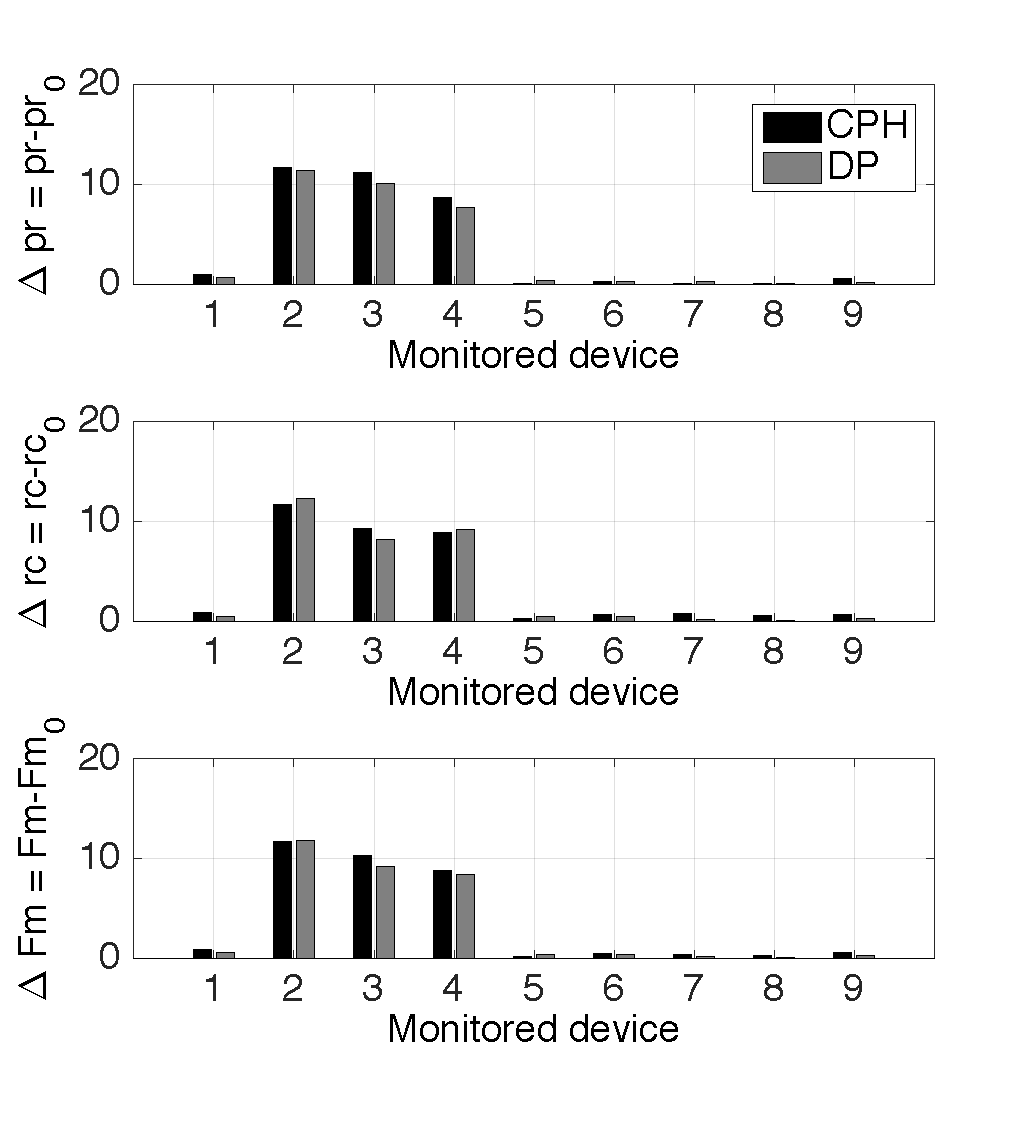
\includegraphics[width=7cm]{./chapters/chapter5/images/R1_kp_1modev.pdf}}
%  \vspace{1.5cm}
  \centerline{(a) REDD 1}\medskip
\end{minipage}
\hfill
\begin{minipage}[b]{.48\linewidth}
  \centering
  \centerline{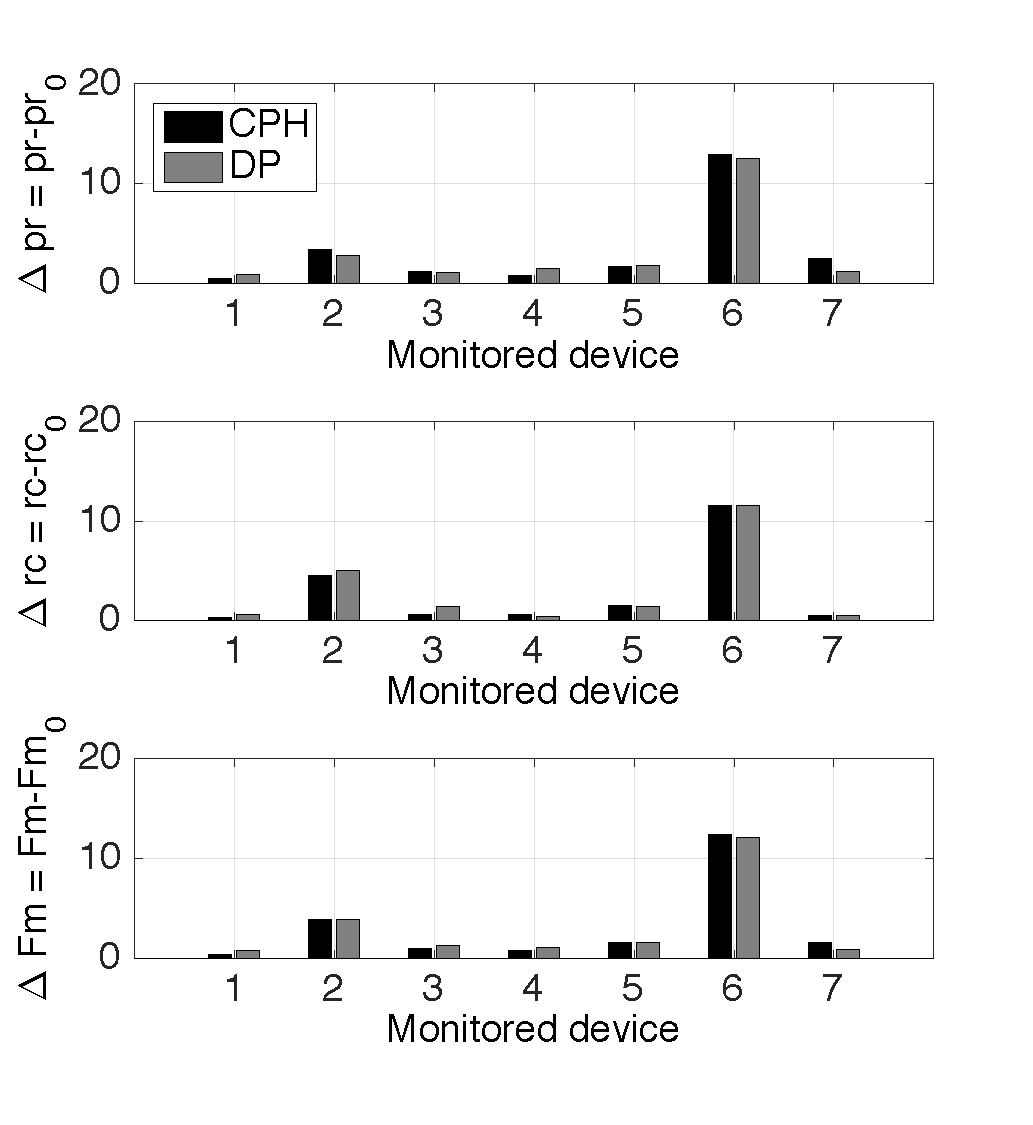
\includegraphics[width=7cm]{./chapters/chapter5/images/R2_kp_1modev.pdf}}
%  \vspace{1.5cm}
  \centerline{(b) REDD 2}\medskip
\end{minipage}
\begin{minipage}[b]{.48\linewidth}
  \centering
  \centerline{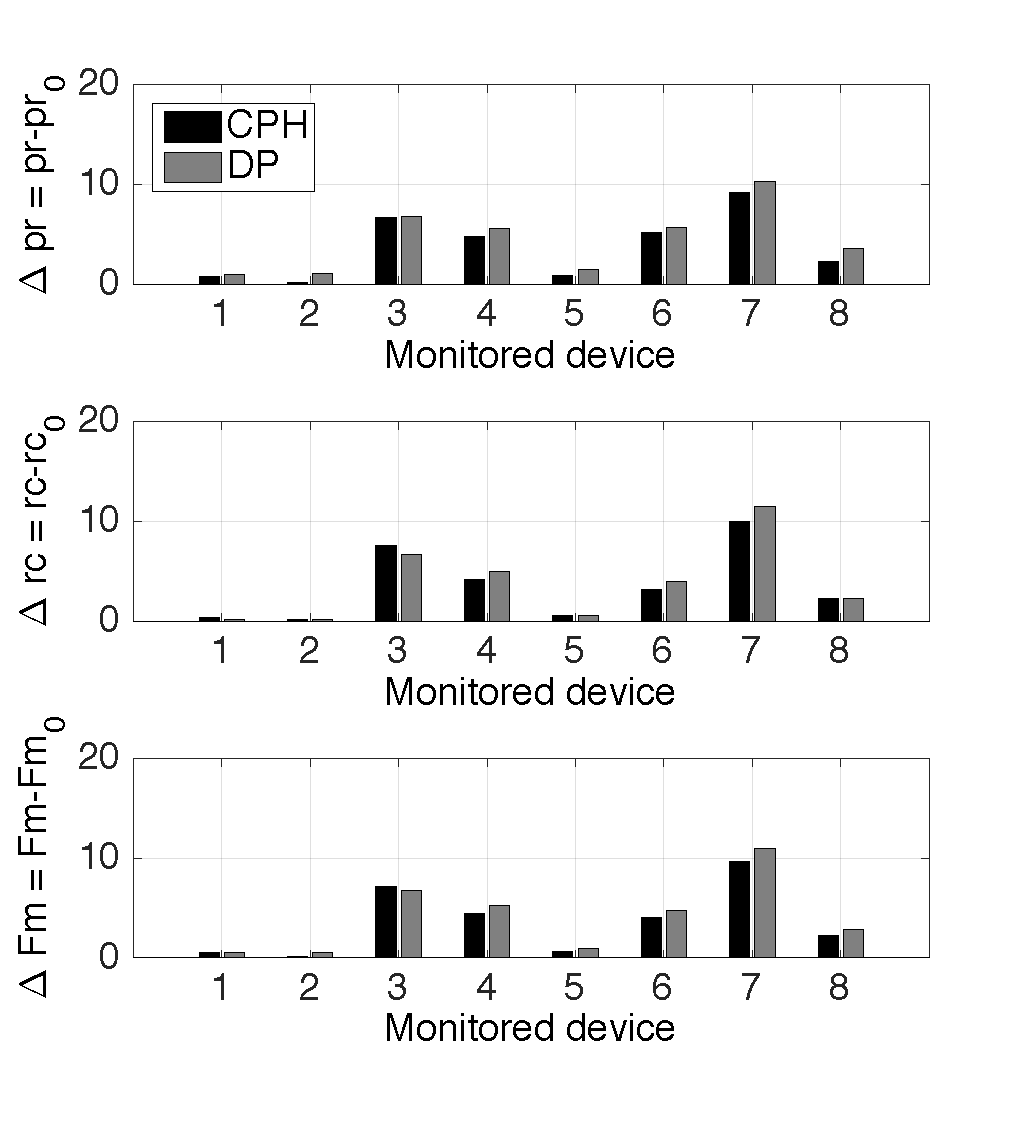
\includegraphics[width=7cm]{./chapters/chapter5/images/UK_kp_1modev.pdf}}
%  \vspace{1.5cm}
  \centerline{(c) UK-DALE 5}\medskip
\end{minipage}
\hfill
\begin{minipage}[b]{0.48\linewidth}
  \centering
  \centerline{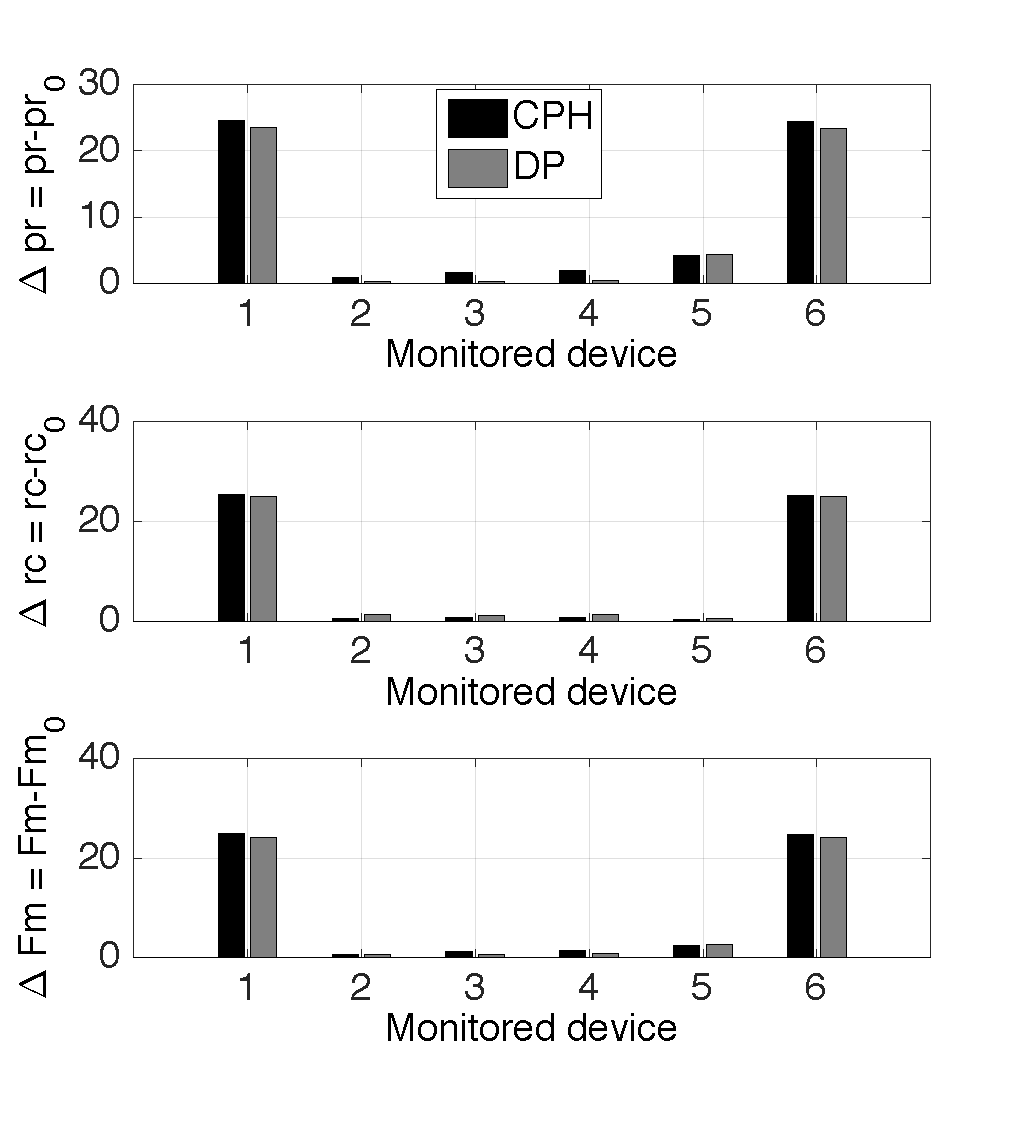
\includegraphics[width=7cm]{./chapters/chapter5/images/A_kp_1modev.pdf}}
%  \vspace{1.5cm}
  \centerline{(d) Athemium}\medskip
\end{minipage}
\caption{Effect of the type of monitored devices on the performance improvement of the CPH and DP algorithms. The values of $pr_0$, $rc_0$, $Fm_0$ correspond to the case without any monitored device, given in Table~\ref{table:SR6}.}
\label{fig:SR1}
%
\end{figure}

\subsection{Implementation results of Optical Network Interface}

In SmartSense, only several specific devices are selected to be monitored, but a relevant question is: Which type of devices can help to improve the performance of the algorithms? In the first experiment, sequentially each device is selected to monitor, the main characteristics of the devices giving the best performance are then analyzed to generalize the criteria to select the monitored devices. 
The precision and recall of the sensors detection are assumed to be equal to $0.9$. Figure~\ref{fig:SR1} shows the performance of the CPH and DP algorithms with different monitored devices in four dataset, in which the labels are respectively noted in Tables \ref{table:SR1}, \ref{table:SR2}, \ref{table:SR3} and \ref{table:SR4}. Because both CPH and DP are searching for the optimal solution, they give similar results.
Table~\ref{table:SR7} lists two devices with the best performance in each dataset. 
In REDD~1, as shown in Figure~\ref{fig:SR1}(a), the best performance corresponds to the fridge with the gain of both precision and recall around 12$\%$. From Table~\ref{table:SR1}, it can be seen that the fridge has a high using rate (24.94$\%$) and its power demand is confused with the dish washer (193W \emph{vs.} 214W). Two other devices also giving a high gain are the dish washer and the lighting system. The lighting system has the largest using rate (48.99$\%$). Although unusually operating, monitoring the dish washer also gives a high performance gain because it consumes a power similar to the fridge. Meanwhile, other devices show a very small gain (<2$\%$) if monitored.
In Figure~\ref{fig:SR1}(b), except for the fridge with the performance improvement over 12$\%$ for all evaluation metrics, deploying the sensors to monitor other devices in REDD~2 can only obtain a gain lower than 5$\%$. This result can be explained from Table~\ref{table:SR2} that besides the most used device (44.40$\%$), the fridge consumes a power very close to the lighting system (163W \emph{vs.} 153W) and stove (426W \emph{vs.} 406W). 
\par Therefore, we can come to a conclusion that the most effective devices to be monitored with CPH and DP algorithms have two main characteristics that are: high using rate and confusion on the power demand with other devices. This conclusion is also consolidated by the results from the UK-DALE~5 and Athemium dataset. As shown in Figure~\ref{fig:SR1}(c), the most effective devices in UK-DALE~5 are the microwave and fridge, which both have high using ratio (68.4$\%$ and 36.48$\%$ respectively) and their power demand is also confused with others. Concretely, the microwave consumes a power close to the washer dryer (1496W and 1492W) and dish washer (49.8W and 57.4W), while the power demand of the fridge is near to the dish washer (109.5W and 96.3W). Meanwhile, in Figure~\ref{fig:SR1}(d), the most effective devices in Athemium dataset are fridge and monitor, which are frequently used (17.79$\%$ and 27.35$\%$ respectively) and their power consumption is also similar (75W and 73W).

\begin{table}
\caption{Most effective devices with the CPH and DP algorithms.}\label{table:SR7}
\begin{center}
\begin{tabular}{|c|c|c|}
\hline
 & CPH & DP \\
 \hline
  \multirow{2}{*}{REDD 1} &2-fridge & 2-fridge \\
 & 3-dish washer & 3-dish washer  \\
 \hline
  \multirow{2}{*}{REDD 2} & 6-fridge & 6-fridge \\
 & 2-lighting & 2-lighting  \\
 \hline
  \multirow{2}{*}{UK-DALE 5} & 7-microwave & 7-microwave\\
  & 3-fridge &3-fridge \\
 \hline
  \multirow{2}{*}{Athemium} & 1-fridge & 1-fridge  \\
 & 6-monitor & 6-monitor  \\
 \hline
\end{tabular}
\end{center}
\end{table}

\begin{figure}[htb]
\begin{minipage}[b]{0.48\linewidth}
  \centering
  \centerline{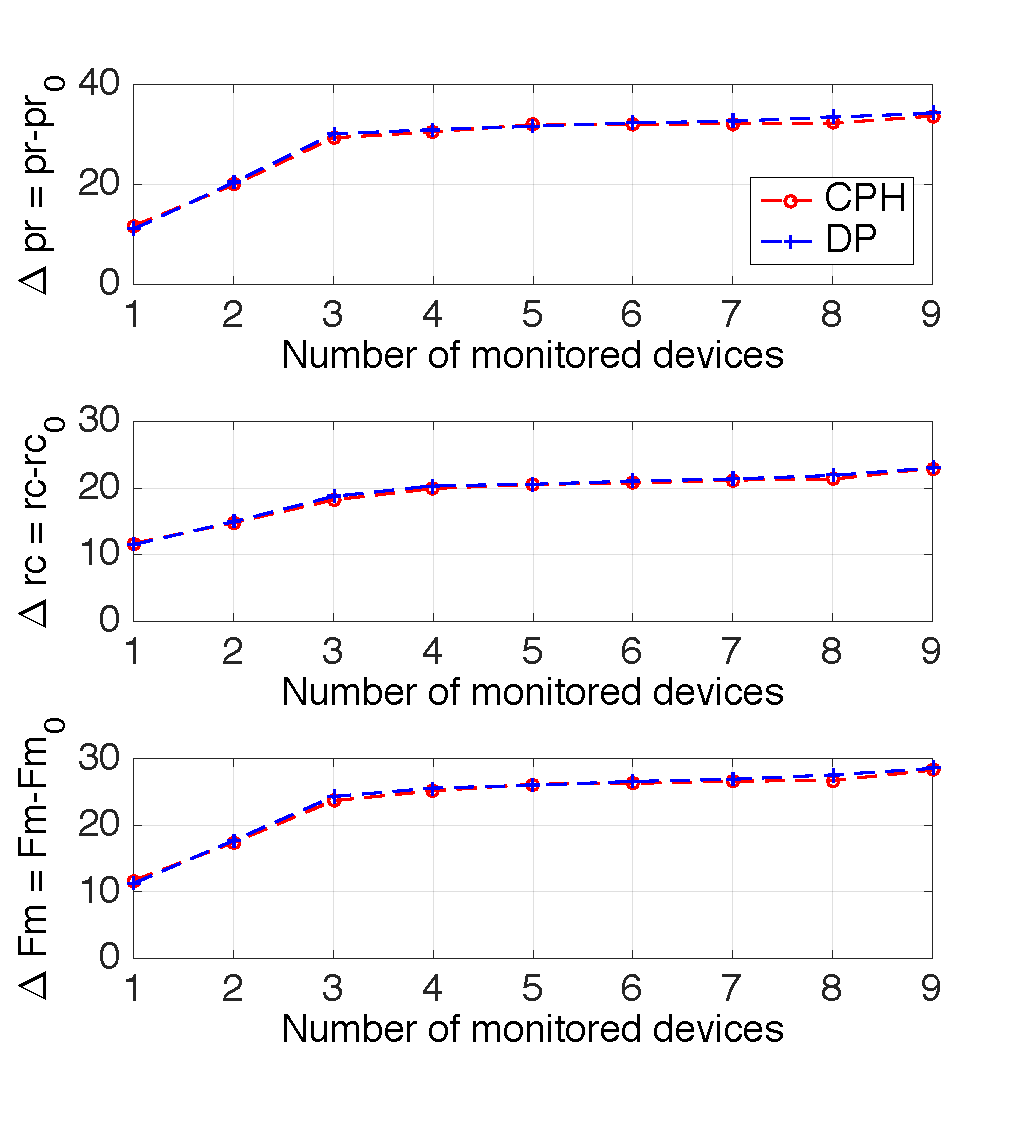
\includegraphics[width=7cm]{./chapters/chapter5/images/R1_kp_nmodev.pdf}}
%  \vspace{1.5cm}
  \centerline{(a) REDD 1}\medskip
\end{minipage}
%
\hfill
\begin{minipage}[b]{.48\linewidth}
  \centering
  \centerline{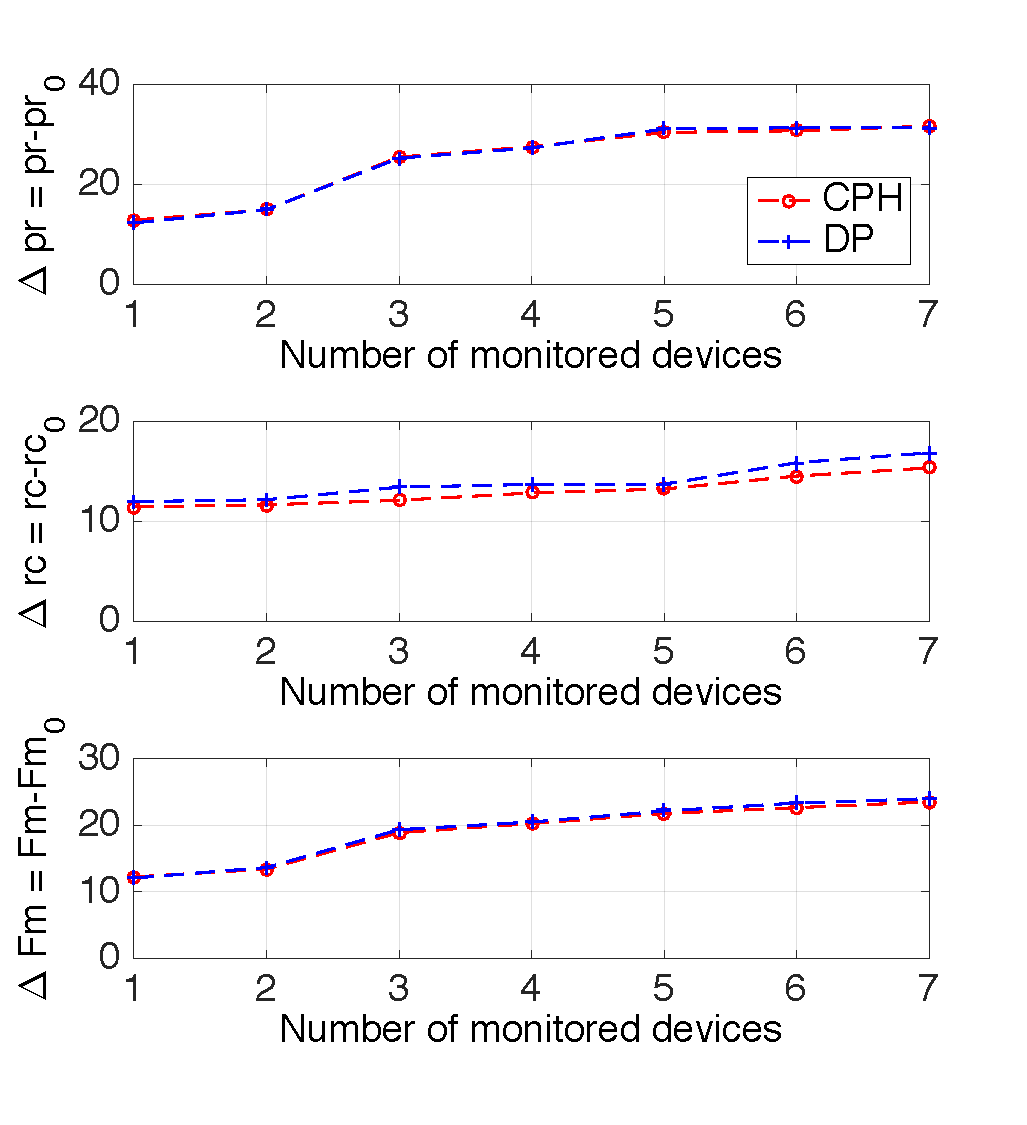
\includegraphics[width=7cm]{./chapters/chapter5/images/R2_kp_nmodev.pdf}}
%  \vspace{1.5cm}
  \centerline{(b) REDD 2}\medskip
\end{minipage}
\begin{minipage}[b]{.48\linewidth}
  \centering
  \centerline{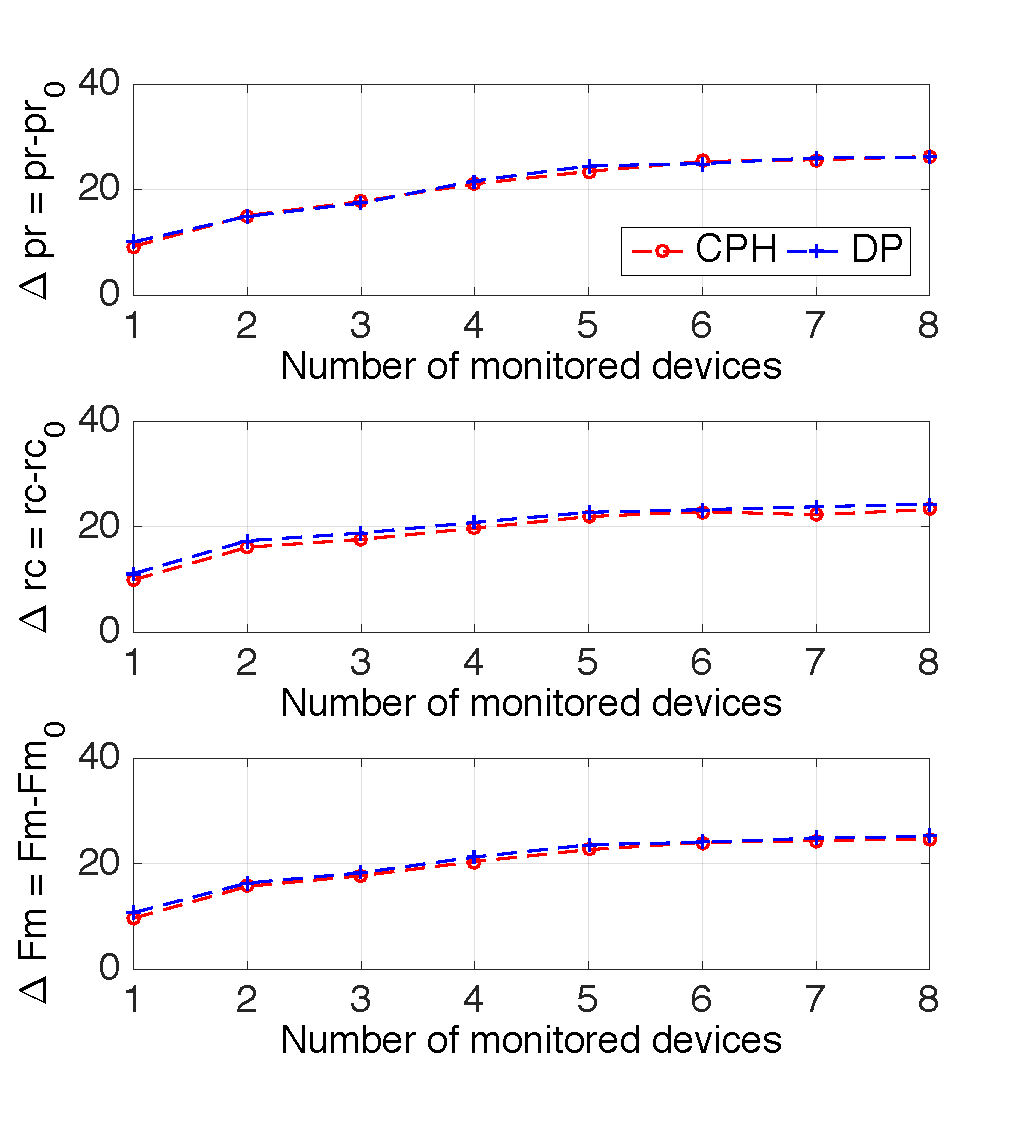
\includegraphics[width=7cm]{./chapters/chapter5/images/UK_kp_nmodev.pdf}}
%  \vspace{1.5cm}
  \centerline{(c) UK-DALE 5}\medskip
\end{minipage}
\hfill
\begin{minipage}[b]{0.48\linewidth}
  \centering
  \centerline{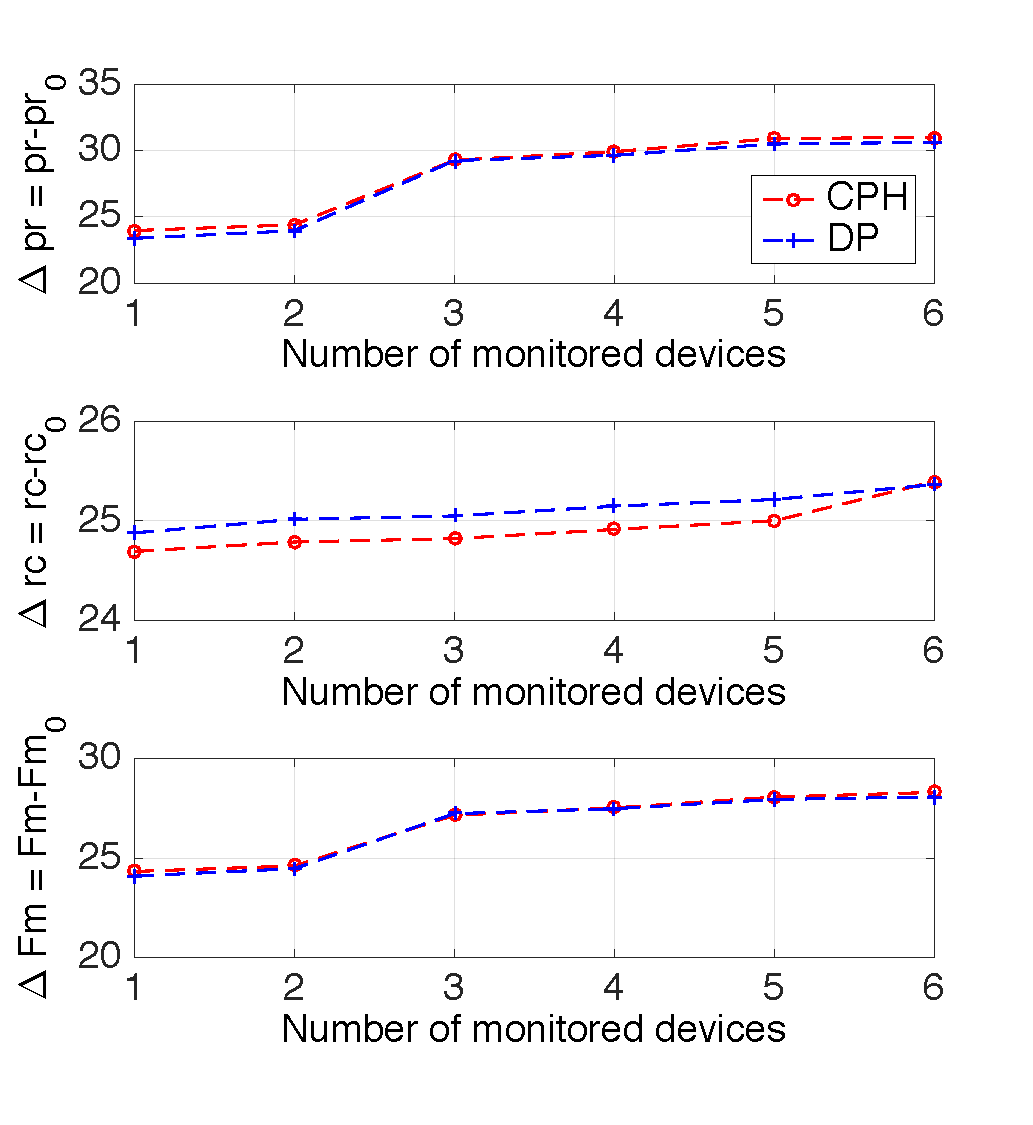
\includegraphics[width=7cm]{./chapters/chapter5/images/A_kp_nmodev.pdf}}
%  \vspace{1.5cm}
  \centerline{(d) Athemium}\medskip
\end{minipage}
\caption{Effect of the number of monitored devices on the performance improvement of the CPH and DP algorithms. The values of $pr_0$, $rc_0$, $Fm_0$ correspond to the case without any monitored device, given in Table~\ref{table:SR6}.}
\label{fig:SR2}
%
\end{figure}

Besides the type, the number of monitored devices is also a parameter strongly affecting on the performance improvement of the algorithms. Apparently, monitoring more devices allows to obtain a better performance. However, the deployment cost also increases along with the size of the monitoring sensors network and the non-intrusive requirement is violated. Therefore, it is necessary to make a trade-off between the size of the WSN and the desired performance when selecting the monitored devices. Figure~\ref{fig:SR2} shows the performance improvement when increasing the number of monitored devices. In each case, the devices are selected based on their performance in Figure~\ref{fig:SR1}. Obviously, there are some devices showing less effectiveness when monitored and adding them to the monitoring list cannot help to significantly improve the performance. Thus, these devices can be ignored when deploying the sensors network. 
Concretely, in REDD~1, three devices giving the best performance are fridge, dish washer and lighting system. Thus, adding these devices to the monitoring list allows to significantly improve the performance of the algorithms. This phenomenon can be illustrated by the slope from one to three devices in Figure~\ref{fig:SR2}(a). The corresponding precision gain increases from 12$\%$ to 30$\%$ and the recall from 11$\%$ to 19$\%$ in this interval. However, other devices are less effective, which results in a slow increase of the performance gain with more than three monitored devices (from 30$\%$ to 37$\%$ with precision and 19$\%$ to 23$\%$ with recall when increasing the number of devices from three to nine).
Similarly, in REDD~2, as shown in Figure~\ref{fig:SR2}(b), the performance is improved very slowly. After monitoring the first device (fridge) and obtaining the precision gain of 13$\%$ and recall gain of 12$\%$, we can only improve the recall around 3$\%$ (from 12$\%$ to 15$\%$) with other six devices added to the monitoring list. Therefore, the F-measure is still insignificant (11$\%$ improved) although the precision gain can be improved from 13$\%$ up to 31$\%$.
Meanwhile, in UK-DALE~5, there are two devices giving a remarkable increase of the performance when monitored including the microwave and fridge, as shown in Figure~\ref{fig:SR1}(c). This is the reason why the performance is significantly improved with the number of monitored devices from one to two, and slowly increased with more other devices.
In contrast, in Athemium dataset, because the fridge and the monitor have only one power state and their power demand are confused together, the performance can be significantly improved by monitoring one of them and it cannot increase anymore if another remaining device is also monitored. This results in the nearly horizontal line from one to two devices in Figure~\ref{fig:SR2}(d). Besides, the performance gain cannot be improved too much when monitoring more other devices.


\begin{figure}[htb]
\begin{minipage}[b]{1\linewidth}
  \centering
  \centerline{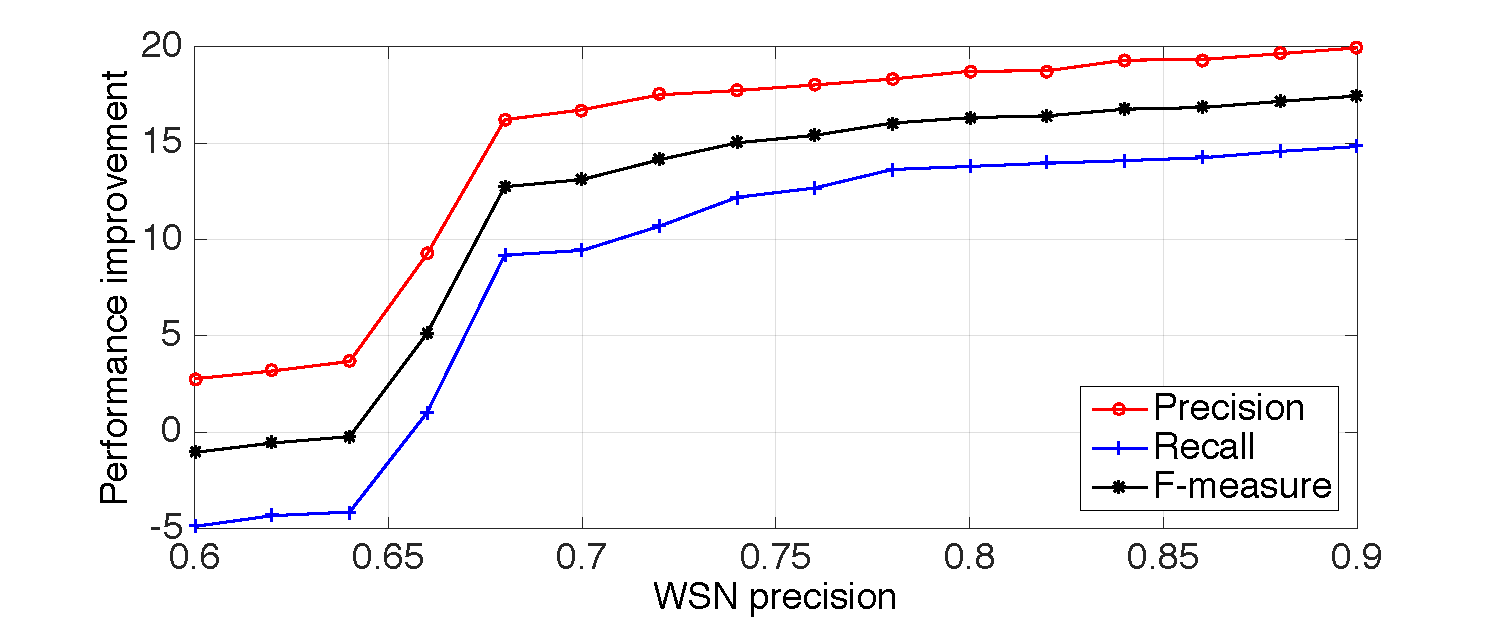
\includegraphics[width=0.75\textwidth]{./chapters/chapter5/images/R1_cph_pr.pdf}}
%  \vspace{1.5cm}
  \centerline{(a) REDD 1}\medskip
\end{minipage}
\hfill
\begin{minipage}[b]{1\linewidth}
  \centering
  \centerline{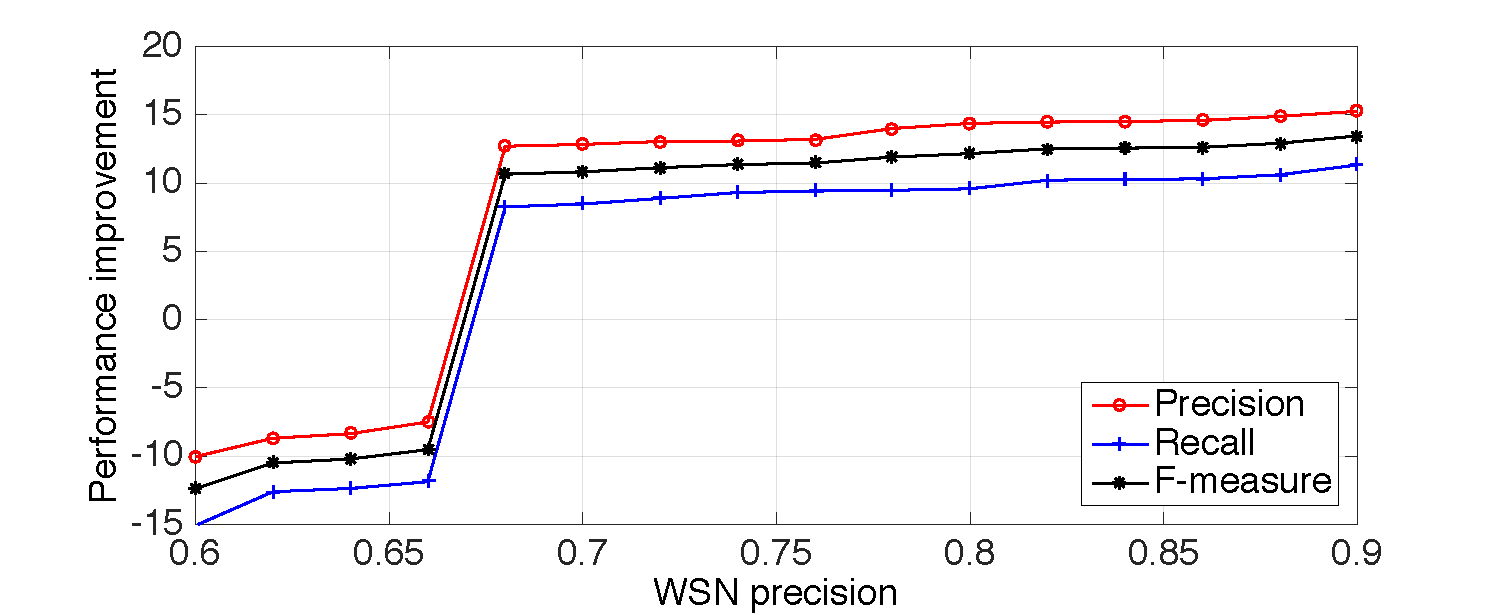
\includegraphics[width=0.75\textwidth]{./chapters/chapter5/images/R2_cph_pr.pdf}}
%  \vspace{1.5cm}
  \centerline{(b) REDD 2}\medskip
\end{minipage}
\caption{Performance improvement of the CPH algorithm when modifying WSN precision.}
\label{fig:SR3}
%
\end{figure}


\begin{figure}[h]
\centering
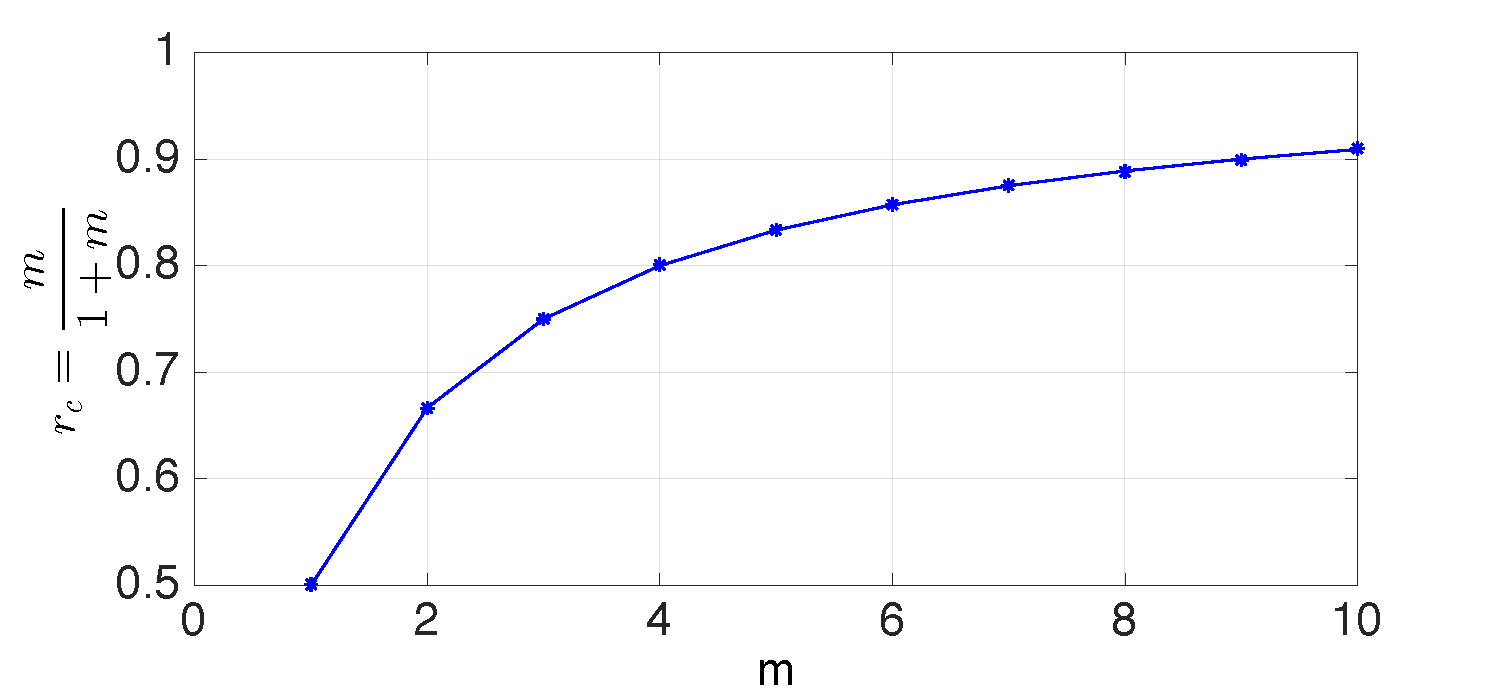
\includegraphics[width=0.65\textwidth]{./chapters/chapter5/images/breakPR.pdf} 
\caption{Dependence of the abnormally changing point on the number of states.} 
\label{fig:SR4} 
\end{figure}







\subsubsection{ECC codecs implementation}

In the experiments above, the WSN is assumed with a detection reliability of $0.9$. However, in real condition, this value can vary depending on the quality of the sensors. Therefore, we will consider the effect of the sensor detection on the overall performance of SmartSense algorithms by tuning the precision from 0.6 to 0.9 with two monitored devices (fridge and dish washer) for REDD~1 and REDD~2. Figure~\ref{fig:SR3} shows the performance gain of the CPH algorithm according to the increase of the WSN precision. 
In Figure~\ref{fig:SR3}(a), with monitored devices, the performance of the algorithm in REDD~1 decreases significantly if the reliability of the sensors is lower than 0.66. This is illustrated by the negative gain of both precision and recall. Meanwhile, when increasing this value from 0.66 to 0.68, the performance abnormally increases with the precision gain from 9$\%$ to 16.5$\%$ and the recall from 1$\%$ to 9$\%$. After this interval, the performance is slowly improved to 20$\%$ of precision gain and 15$\%$ of recall gain at a WSN precision of 0.9.
Similarly, with REDD~2, as shown in Figure~\ref{fig:SR3}(b), the performance gain is also negative with the WSN reliability less than 0.6 and there also exists an abnormally changing interval between 0.66 and 0.68, in which the precision gain increases from -7.5$\%$ to 12.5$\%$ and the recall from -12$\%$ to 8$\%$. Beyond this interval, the performance slowly increases along with the WSN precision.
To find the reason of the abnormally increasing interval, let return to Section~\ref{knapsack}. If an $m$-state device is detected as switched on, the corresponding probability of each power state is equal to $pr/m$ and off-state is $(1-pr)$. Thus, with $pr<m/(m+1)$, the probability of the off-state is greater than any on-state although the device is operating and that makes the decrease of performance. In contrast, if $pr>m/(m+1)$, the probability of any on-state is larger than off-state and the probability information allows to improve the detection accuracy. In both REDD~1 and REDD~2 dataset, the monitored devices are fridge and dish washer, each of which has two operation states, which creates a changing point at $pr\approx 0.67$. Obviously, with the edge detector approach, this phenomenon always happens at $pr = 0.5$. 
The dependence of the changing point $pr=\frac{m}{m+1}$ on the number of states of devices is presented in Figure~\ref{fig:SR4}. \par As a consequence, the reliability of the WSN needs to ensure to stay on the upper plane discriminated by the changing curve in order to allow the algorithm to reach a better performance. 










\begin{figure}[htb]
\begin{minipage}[b]{0.48\linewidth}
  \centering
  \centerline{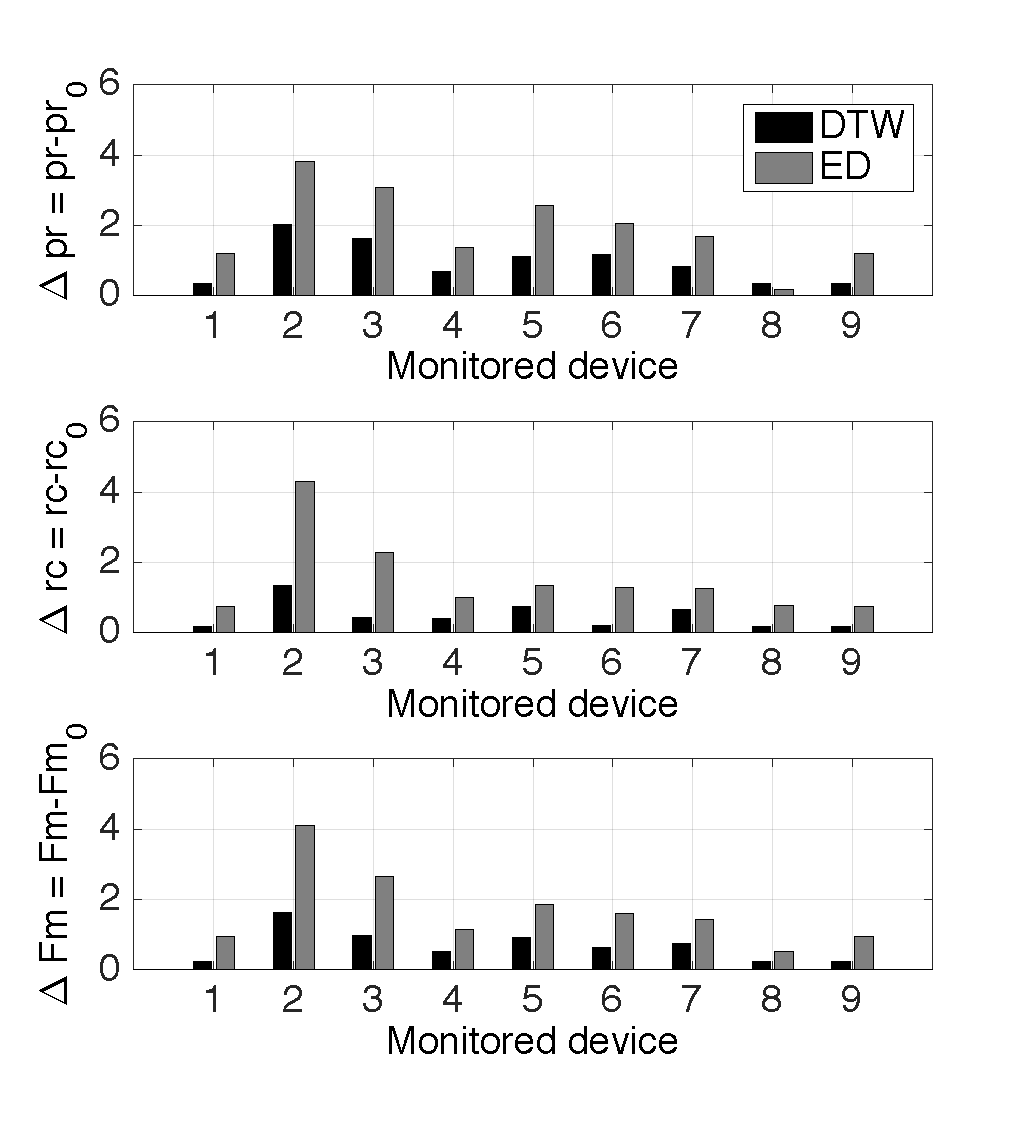
\includegraphics[width=7cm]{./chapters/chapter5/images/R1_ed_1modev.pdf}}
%  \vspace{1.5cm}
  \centerline{(a) REDD 1}\medskip
\end{minipage}
%
\hfill
\begin{minipage}[b]{.48\linewidth}
  \centering
  \centerline{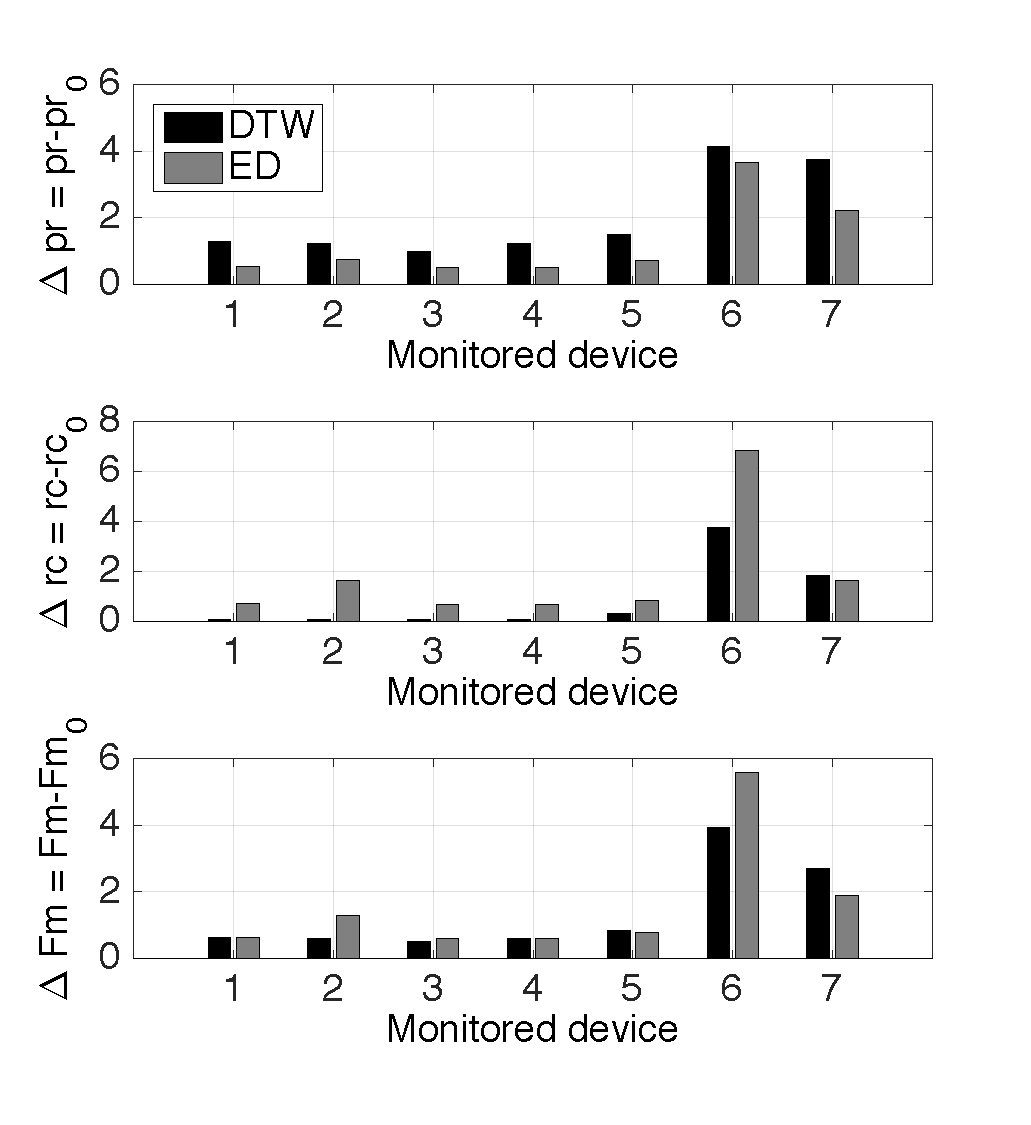
\includegraphics[width=7cm]{./chapters/chapter5/images/R2_ed_1modev.pdf}}
%  \vspace{1.5cm}
  \centerline{(b) REDD 2}\medskip
\end{minipage}

\caption{Effect of the type of monitored devices on the performance improvement of the DTW and ED algorithms. The values of $pr_0$, $rc_0$, $Fm_0$ correspond to the case without any monitored device, given in Table~\ref{table:SR6}.}
\label{fig:SR5}
%
\end{figure}



\subsubsection{Serializer -- Deserializer implementation}

Similar to CPH and DP algorithms, the performance of the DTW and ED algorithms in SmartSense also depends on the type of monitored devices. To analyze the main characteristics of the most effective devices, each device in REDD~1 and REDD~2 is sequentially selected to monitored. The performance gain compared with the original algorithms in NILM, given in Table~\ref{table:SR6}, is shown in Figure~\ref{fig:SR5}. Two devices in each dataset giving the best gain are listed in Table~\ref{table:SR8}.
As shown in Figure~\ref{fig:SR5}(a), the fridge is the best effective device to be monitored in REDD~1. By applying the ED algorithm, monitoring the fridge can achieve a precision gain of 4$\%$ and recall gain of 4.2$\%$. Comparing with Table~\ref{table:SR2}, because the fridge has the confusion on the power demand with the dish washer, both devices have a near value of edge height, which reduces the performance of the edge detector based algorithms in a traditional NILM system. By monitoring one of them, the ambiguity can be overcome. Besides, the fridge also has a high number of activations during the observation period (1695 times). Obviously, monitoring the devices with high number of uses allows to increase the overall performance of the algorithms. The second largest gain in REDD~1 corresponds to the dish washer with 3$\%$ and 2$\%$ for the gain of precision and recall, respectively. Besides confused with the fridge on the edges height, this device is also frequently switched on/off. 
Meanwhile, the performance improvement given by the DTW algorithm is lower then the ED one with only 2$\%$ of precision gain and 1.4$\%$ of recall gain when monitoring the fridge. The respective results for the dish washer are 1.9$\%$ and 0.25$\%$. The small gain of the DTW algorithm with this dataset can be explained by the fact that it shows a good performance without any monitored device ($pr=83.53\%$, $rc=76.48\%$) and it is difficult to improve its performance.
In REDD~2, as shown in Figure~\ref{fig:SR5}(b), the best gain also corresponds to the fridge with 3.9$\%$ of precision and 6.9$\%$ of recall with ED algorithm. The respective values with DTW method are 4.05$\%$ and 3.9$\%$. Similar to REDD~1, the fridge in REDD~2 is also the most frequently used device and its edges are also ambiguous with the lighting system (153W) and dish washer (426W) when it changes the state from 163W to 426W with a rising edge of 263W. This is also the reason why the dish washer is the second effective device in this dataset.
From the results in Figure~\ref{fig:SR5}, it can be concluded that the edge detector based algorithms are sensible with the devices more frequently switched on/off and having the confusion on the edges height (correlated to the power demand) with the others. Therefore, it is necessary to analyze these two characteristics to select the effective monitored devices.

\begin{figure}[htb]

\begin{minipage}[b]{0.48\linewidth}
  \centering
  \centerline{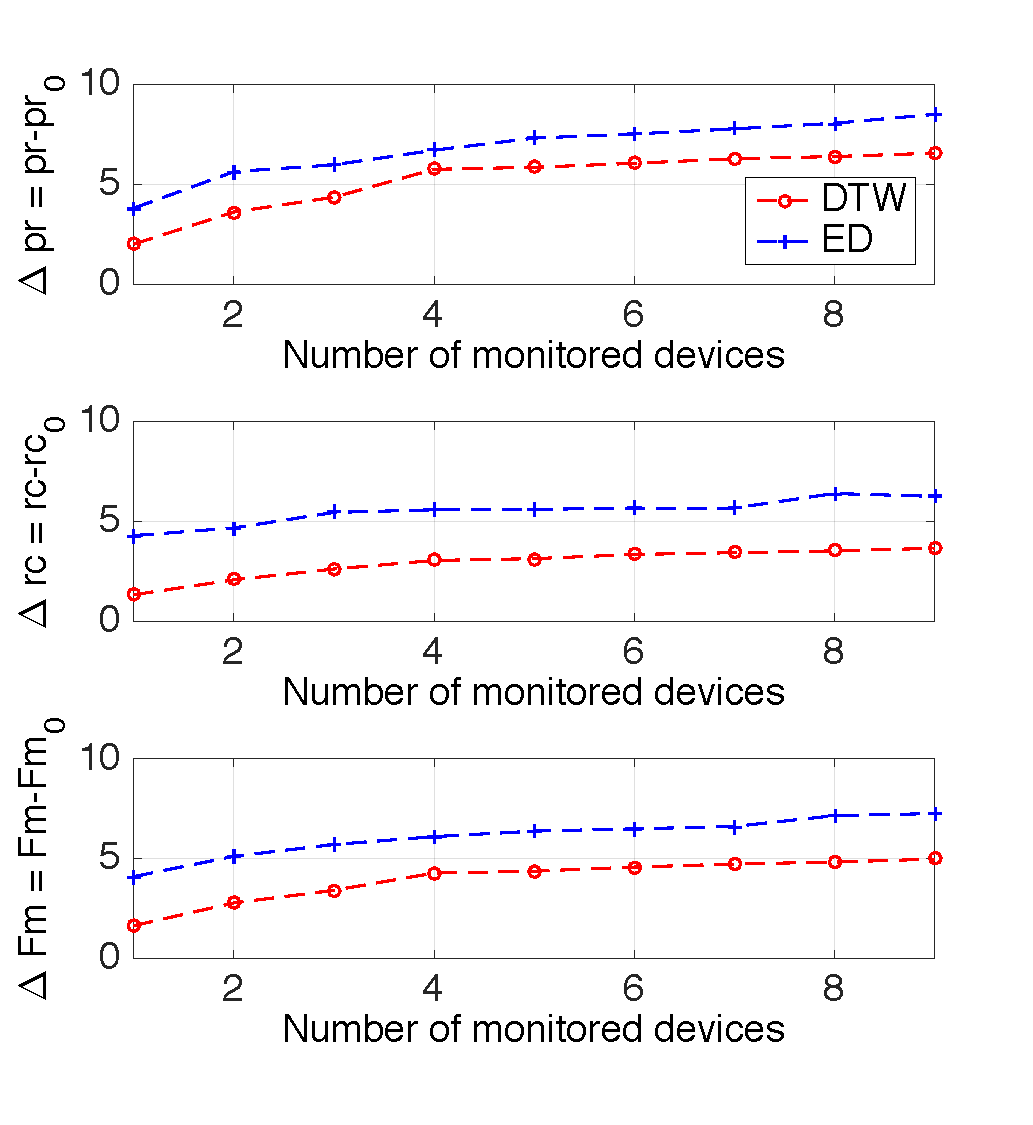
\includegraphics[width=7cm]{./chapters/chapter5/images/R1_ed_nmodev.pdf}}
%  \vspace{1.5cm}
  \centerline{(a) REDD 1}\medskip
\end{minipage}
%
\hfill
\begin{minipage}[b]{.48\linewidth}
  \centering
  \centerline{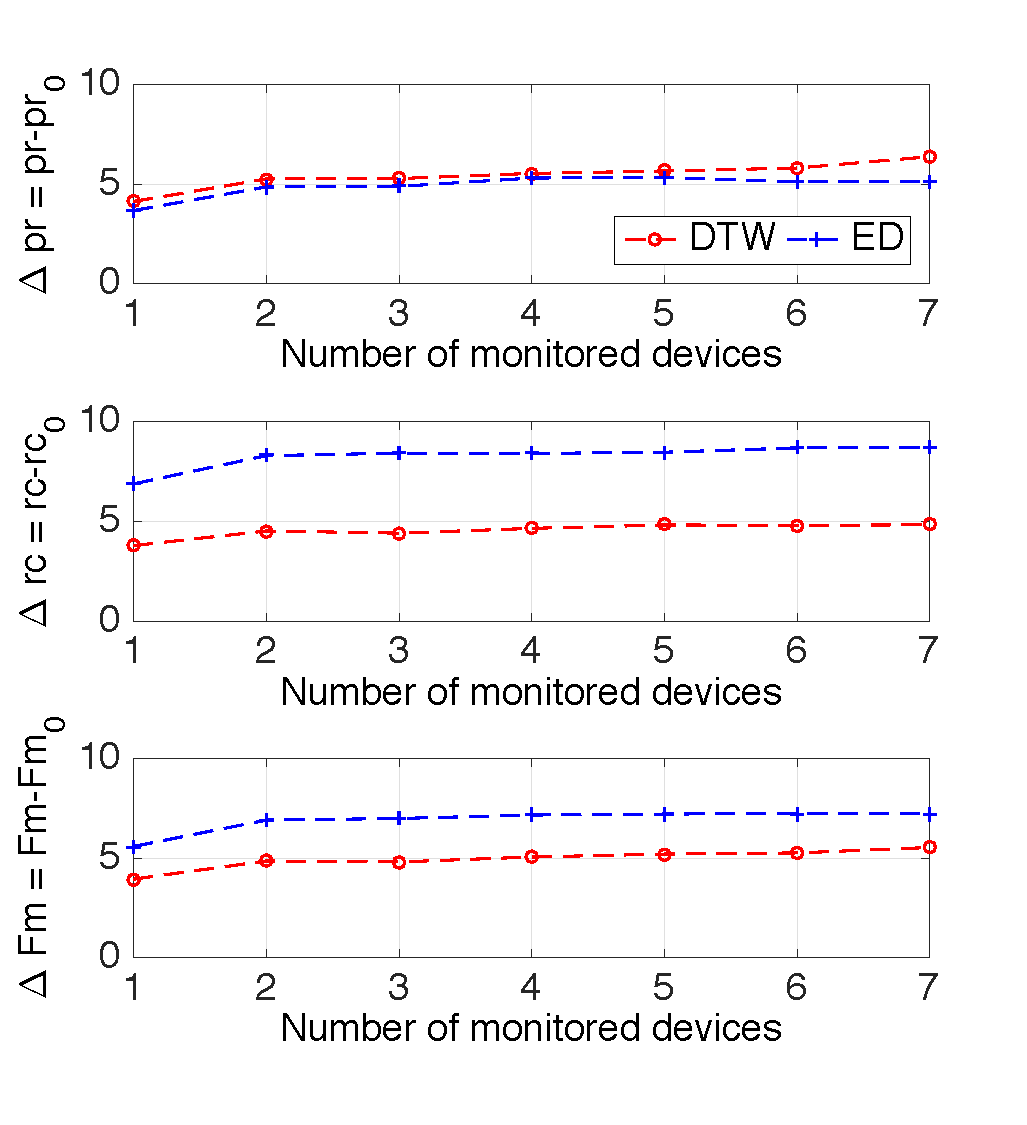
\includegraphics[width=7cm]{./chapters/chapter5/images/R2_ed_nmodev.pdf}}
%  \vspace{1.5cm}
  \centerline{(b) REDD 2}\medskip
\end{minipage}
\caption{Effect of the number of monitored devices on the performance improvement of the DTW and ED algorithms. The values of $pr_0$, $rc_0$, $Fm_0$ correspond to the case without any monitored device, given in Table~\ref{table:SR6}.}
\label{fig:SR6}
%
\end{figure}


\begin{table}
\caption{Most effective devices with DTW and ED algorithms.}\label{table:SR8}
\begin{center}
\begin{tabular}{|c|c|c|}
\hline
& DTW & ED\\
\hline
\multirow{2}{*}{REDD 1} & 2-fridge &2-fridge \\
& 3-dish washer & 3-dish washer \\
\hline
\multirow{2}{*}{REDD 2}  & 6-fridge&6-fridge \\
& 7-dish washer&7-dish washer \\
\hline
\end{tabular}
\end{center}
\end{table}
\subsubsection{Allocator implementation}
The performance gain also slowly increases when adding more devices to the monitoring list, as illustrated in Figure~\ref{fig:SR6}. In this results, the monitored devices are selected based on their performance in Figure~\ref{fig:SR5}. In Figure~\ref{fig:SR6}(a), with two monitored devices (fridge and dish washer) in REDD~1, the precision of the ED algorithm can be improved by 6$\%$ and the recall by 5$\%$. Meanwhile, with other additional devices, the precision can only increase by 2.8$\%$ (from 6$\%$ to 8.8$\%$) and the recall by 1.5$\%$ (from 5$\%$ to 6.5$\%$). Similarly, in REDD~2 as shown in Figure~\ref{fig:SR6}(b), the performance gain obtainable with the ED algorithm is 5$\%$ of precision and 8.5$\%$ of recall with only fridge and dish washer monitored. Then, it increases very slowly when adding more devices to the monitoring list. Concretely, the precision gain increases from 5$\%$ to 6.5$\%$ and the recall from 8.5$\%$ to 9$\%$ with the number of devices from two to seven. Therefore, it is necessary to evaluate the efficiency of each device in improving the overall performance before deploying the monitoring sensors.

\begin{figure}[htb]
\begin{minipage}[b]{1\linewidth}
  \centering
  \centerline{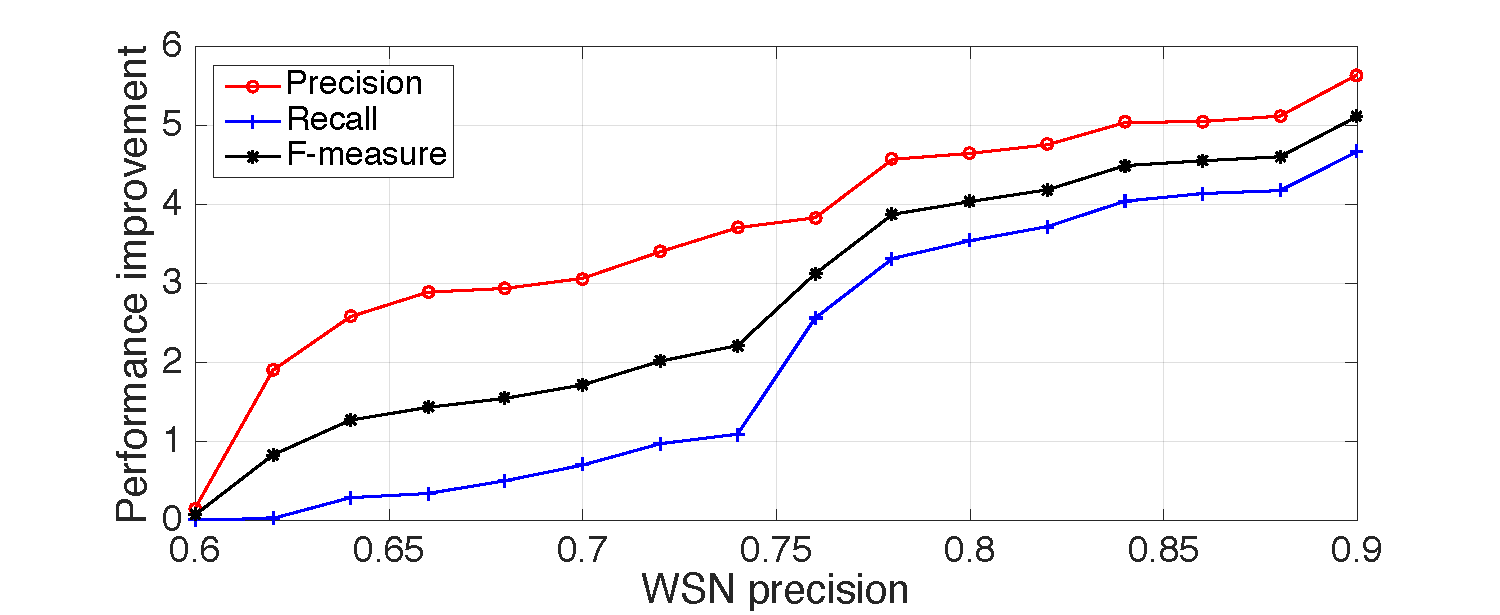
\includegraphics[width=0.75\textwidth]{./chapters/chapter5/images/R1_ed_pr.pdf}}
%  \vspace{1.5cm}
  \centerline{(a) REDD 1}\medskip
\end{minipage}
\hfill
\begin{minipage}[b]{1\linewidth}
  \centering
  \centerline{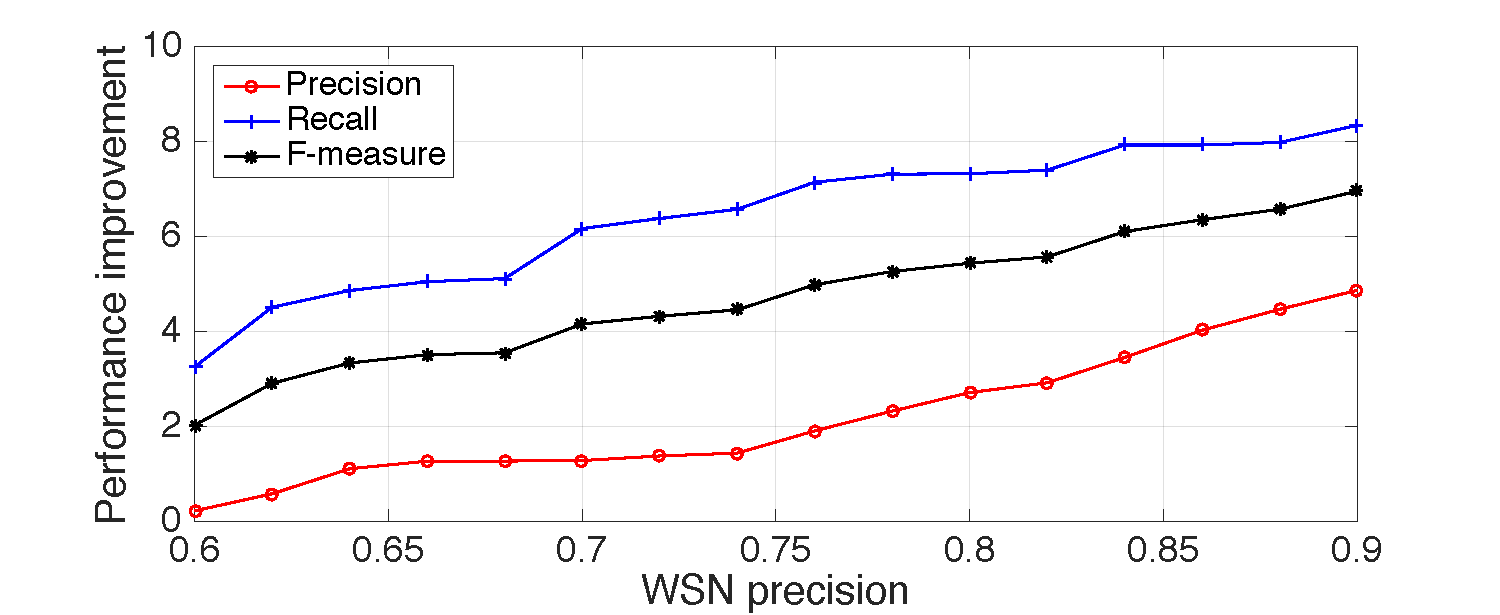
\includegraphics[width=0.75\textwidth]{./chapters/chapter5/images/R2_ed_pr.pdf}}
%  \vspace{1.5cm}
  \centerline{(b) REDD 2}\medskip
\end{minipage}
\caption{Performance improvement of the ED algorithm versus the WSN precision.}
\label{fig:SR7}
%
\end{figure}

Similar to CPH and DP, the performance of the edge detector based algorithms also increases along with the increase of the WSN detection precision, as illustrated by the simulation results of ED one with REDD~1 and REDD~2 in Figure~\ref{fig:SR7}. Because the operating probability of each device is not divided by the number of states, there is only one abnormally changing point at $pr=0.5$ for these algorithms. This point is not presented in Figure~\ref{fig:SR7} because the value of WSN precision is only tuned from 0.6 to 0.9. Moreover, a WSN precision of 0.5 is equivalent to a random selection of the state, which is not relevant in our case.





\subsection{Communication time and latency}
\begin{figure}[htb]

\begin{minipage}[b]{1\linewidth}
  \centering
  \centerline{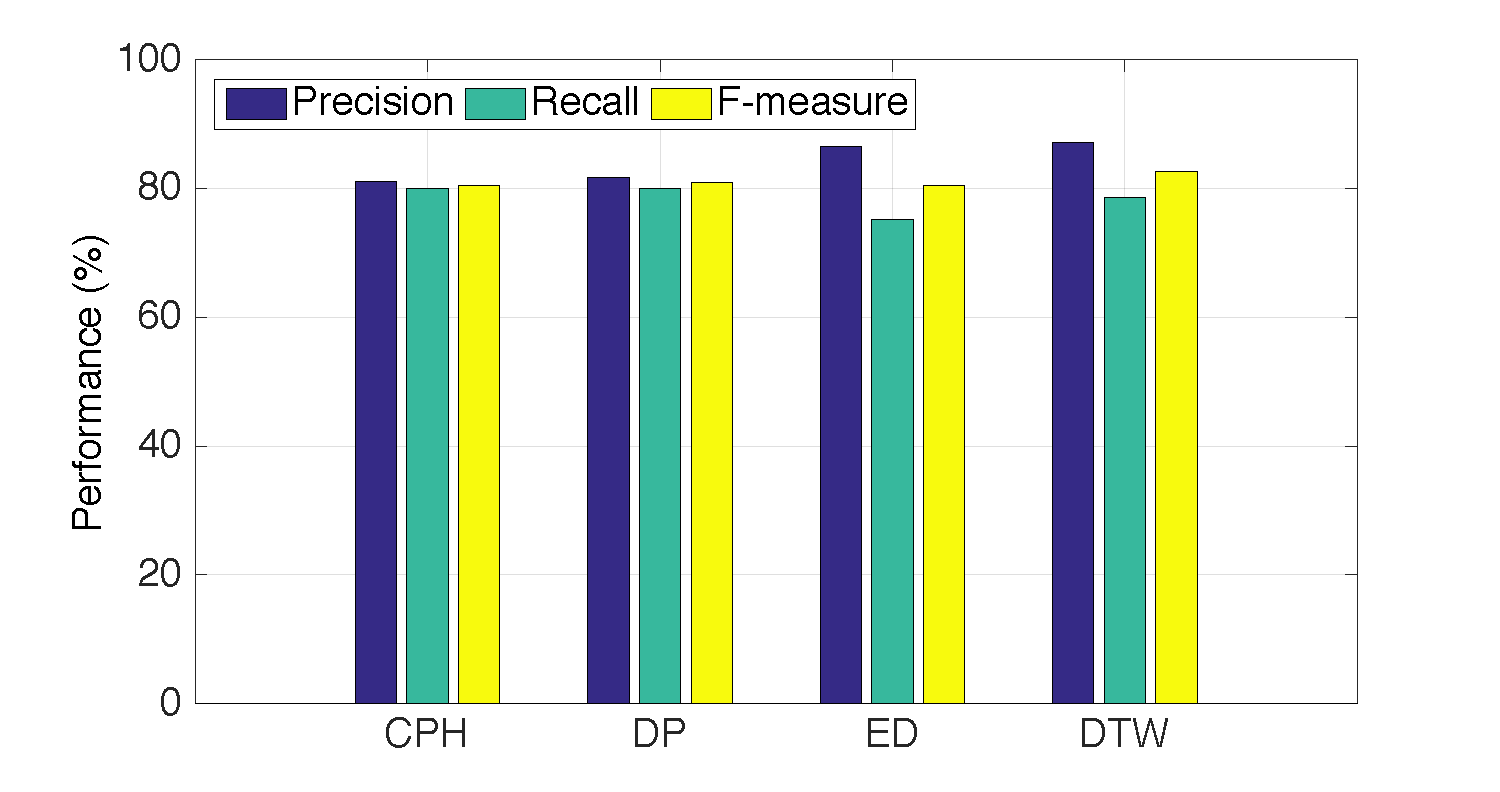
\includegraphics[width=.75\textwidth]{./chapters/chapter5/images/R1_perfcom.pdf}}
%  \vspace{1.5cm}
  \centerline{(a) REDD 1}\medskip
\end{minipage}
%
\hfill
\begin{minipage}[b]{1\linewidth}
  \centering
  \centerline{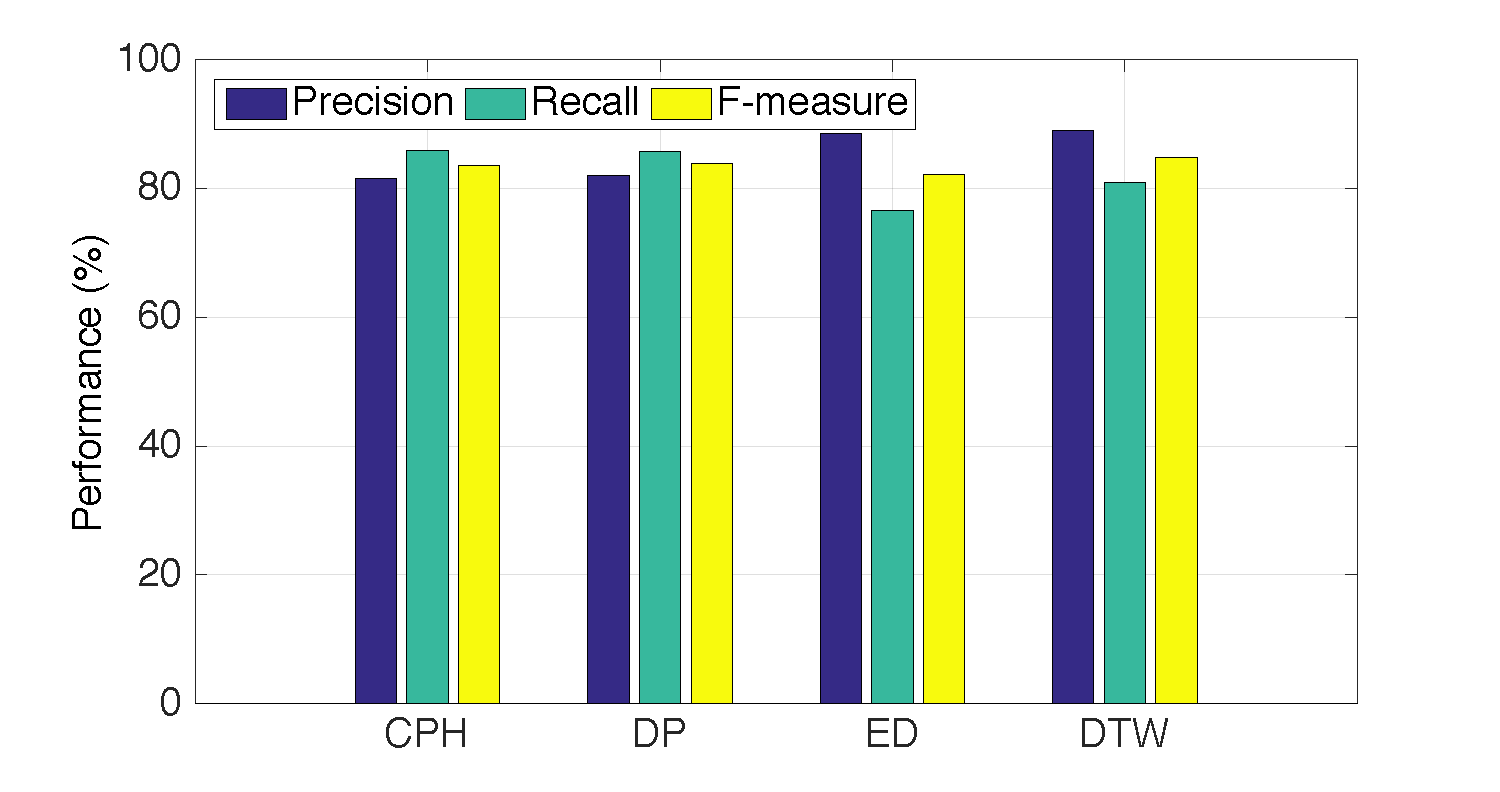
\includegraphics[width=.75\textwidth]{./chapters/chapter5/images/R2_perfcom.pdf}}
%  \vspace{1.5cm}
  \centerline{(b) REDD 2}\medskip
\end{minipage}
\caption{Performance comparison of the proposed algorithms with two monitored devices.}
\label{fig:SR8}
%
\end{figure}

Comparing with the CPH and DP methods, it can be noticed that the improvement of the DTW and ED algorithms is much lower. As presented in Table~\ref{table:SR6}, these algorithms show high performance without monitored device. Concretely, the F-measure of the ED algorithm is greater than 75$\%$ and the DTW one over 79$\%$. Meanwhile, the CPH and DP algorithms can only show an F-measure lower than 70$\%$. Obviously, high performance prevents the edge detector based algorithms from giving a high gain. In addition, the results also come from the fact that performance of these algorithms also depends on the edge detector capacity. Therefore, despite outperforming the algorithms with the knapsack approach in a traditional NILM system, both DTW and ED algorithms can only show a near performance in term of F-measure with two monitored devices, as illustrated in Figure~\ref{fig:SR8}. Of course, comparing the increase of the gain in Figures~\ref{fig:SR2} and \ref{fig:SR6}, the CPH and DP algorithms can show a better performance than the ED and DTW ones with more than two monitored devices in home.
Besides the overall performance, the performance per device of each proposed algorithms with two monitored devices for each dataset (selected by the results in Figure~\ref{fig:SR1} for CPH and DP algorithms and Figure~\ref{fig:SR5} for ED and DTW ones) is also presented in Tables~\ref{table:SR9}, \ref{table:SR10}, \ref{table:SR11} and \ref{table:SR12}, respectively.

\begin{table}
\caption{Performance per device in REDD~1 ($\%$).}\label{table:SR9}
\begin{center}
\begin{tabular}{|c|c|c|c|c|c|c|c|c|c|c|}
\hline
\multicolumn{2}{|c|}{Device}& 1&2&3&4&5&6&7&8&9\\
\hline
\multirow{3}{*}{CPH} & $pr$ &65.08 &97.66 &86.64 &78.55 &41.69 &19.23 &22.77 &30.14 &97.16 \\
& $rc$ & 36.80&88.95 &87.66 &79.28 &46.53 &45.17 &35.11 &29.46 &69.22  \\
& $Fm$ &47.01 &93.10 &87.15 &78.91 &43.97 &26.98 &27.63 &29.79 &80.84 \\
\hline
\multirow{3}{*}{DP} & $pr$ & 63.94&99.16 &96.50 &76.55 &43.79 &22.50 &20.63 &19.91 &94.68 \\
& $rc$ &35.84 &91.59 &92.13 &76.00 &41.20 &46.26 &42.84 &25.71 &73.34  \\
& $Fm$ &45.93 &95.23 &94.26 &76.27 &42.45 &30.28 &27.85 &22.44 &82.66 \\
\hline
\multirow{3}{*}{ED} & $pr$ &42.88 &93.65 &95.81 &61.91 &31.33 &40.52 &49.27 &21.17 &99.75 \\
& $rc$ &59.66 &80.43 &83.88 &61.35 &68.01 &61.91 &43.21 &19.12 &54.18  \\
& $Fm$ &49.89 & 86.54 & 89.45 & 61.63 &42.90 & 48.98 &46.04 & 20.09 & 70.72 \\
\hline
\multirow{3}{*}{DTW} & $pr$ &47.54 &89.35 &80.85 &68.81 &34.17 &87.41 &94.36 &21.46 &99.36 \\
& $rc$ &74.95 &85.90 &86.19 & 25.05&68.01 &65.17 &60.77 &20.45 &67.61  \\
& $Fm$ &58.18 &87.59 &83.43 &36.73 &45.48 &74.67 &73.93 &20.94 &40.47 \\
\hline
\end{tabular}
\end{center}
\end{table}

\begin{table}
\caption{Performance per device in REDD~2 ($\%$).}\label{table:SR10}
\begin{center}
\begin{tabular}{|c|c|c|c|c|c|c|c|c|}
\hline
\multicolumn{2}{|c|}{Device}& 1&2&3&4&5&6&7\\
\hline
\multirow{3}{*}{CPH} & $pr$ &23.10 &91.60 &27.17 &99.25 &62.23 &99.92 &27.42  \\
& $rc$ & 24.20& 86.62&85.80 &30.73 &56.47 &92.86 &55.58  \\
& $Fm$ & 23.64&89.04 &41.27 &46.94 &59.21 &96.26 &36.72  \\
\hline
\multirow{3}{*}{DP} & $pr$ & 27.18&95.53 &26.02 &97.33 &48.57 &99.95 &26.82 \\
& $rc$ & 43.19&90.49 &86.80 &21.84 &38.09 &88.44 &57.10   \\
& $Fm$ &33.36 &92.94 &40.04 &35.67 &42.70 &93.85 &36.50  \\
\hline
\multirow{3}{*}{ED} & $pr$ & 80.65 &94.05 &21.55 &100 & 63.09 &85.60 &82.71\\
& $rc$ &19.65 & 41.75 & 99.13 & 17.62 & 85.12 & 85.96 & 84.43   \\
& $Fm$ & 31.60 & 57.82 & 35.40 & 29.96 & 72.47 & 85.78 & 83.56  \\
\hline
\multirow{3}{*}{DTW} & $pr$ & 81.56& 95.07 &21.55 & 52.71& 63.09&84.37&80.54 \\
& $rc$ & 29.46&43.19 &93.13 &39.64 &85.12 &90.27 &83.92  \\
& $Fm$ &43.29 &59.40 &35.01 &45.62 &72.47 &87.22 &82.19  \\
\hline
\end{tabular}
\end{center}
\end{table}

\begin{table}
\caption{Performance per device in UK-DALE~5 ($\%$).}\label{table:SR11}
\begin{center}
\begin{tabular}{|c|c|c|c|c|c|c|c|c|c|}
\hline
\multicolumn{2}{|c|}{Device}& 1&2&3&4&5&6&7&8\\
\hline
\multirow{3}{*}{CPH} & $pr$ &22.83 &36.99 &91.24 &40.35 & 17.48 &22.15 &97.46 &87.10 \\
& $rc$ &69.10 &55.31 &89.88 &24.74 &52.20 &67.68 &85.72 &75.84  \\
& $Fm$ &34.32 &44.33 &90.55 &30.67 &26.19 &33.38 &91.21 &81.08 \\
\hline
\multirow{3}{*}{DP} & $pr$ &23.57 &40.77 &90.57 &37.47 &25.81 &23.08 &98.31 &88.52 \\
& $rc$ &58.02 &80.19 &89.15 &22.66 &53.18 &72.60 &87.45 &65.03  \\
& $Fm$ & 33.52&54.08 &89.86 &28.24 &34.75 &35.02 &92.56 &74.98 \\
\hline
\end{tabular}
\end{center}
\end{table}

\begin{table}
\caption{Performance per device in Athemium dataset ($\%$).}\label{table:SR12}
\begin{center}
\begin{tabular}{|c|c|c|c|c|c|c|c|c|c|}
\hline
\multicolumn{2}{|c|}{Device}& 1&2&3&4&5&6\\
\hline
\multirow{3}{*}{CPH} & $pr$ & 93.55 & 86.17& 98.91 &65.31 &85.73 &99.16 \\
& $rc$ &99.14 &99.16 &81.69 &80.41 &98.61 &95.01  \\
& $Fm$ &96.27 &92.21 &89.48 &72.08 &91.72 &97.04  \\
\hline
\multirow{3}{*}{DP} & $pr$ & 86.43 &89.73 &100 &65.60 &82.63 &99.41 \\
& $rc$ & 99.46&99.16 &91.09 &87.80 &98.89 &87.92   \\
& $Fm$ & 92.49&94.21 &95.34 &75.09 &90.03 &93.31 \\
\hline
\end{tabular}
\end{center}
\end{table}

Apparently, the detection of the monitored devices is significantly improved.  For example in REDD~1, as in Table~\ref{table:SR9}, both fridge (2) and dish washer (3) are identified with the precision and recall greater than 85$\%$ by the CPH and DP algorithms and over 80$\%$ by the edge detector ones. Concretely, without sensors, the performance of the CPH algorithm with the fridge is only 62.13$\%$ of precision and 57.78$\%$ of recall as shown in Table~\ref{table:SR6a}, but they are significantly improved up to 97.66$\%$ and 88.95$\%$, respectively, in SmartSense. Similarly, the reliability of detecting the dish washer also increases from 23.83$\%$ to 81.64$\%$ and the sensibility increases from 69.28$\%$ to 87.66$\%$. Meanwhile, the precision of the DTW approach increases from 85.39$\%$ to 89.35$\%$ when detecting the fridge and from 78.85$\%$ to 80.85$\%$ when detecting the dish washer. The respective recall is from 83.49$\%$ to 85.9$\%$ and from 56.19$\%$ to 86.19$\%$. The performance improvement of the monitored devices in other dataset is similar.
In SmartSense, not only the detection of the monitored devices but the identification of other loads is also improved. It comes from the fact that in each dataset, these loads have confusions on the power demand with the monitored ones and the additional information in SmartSense helps to overcome this ambiguity.
For example in REDD~2, referring to Tables~\ref{table:SR6b} and \ref{table:SR10}, the performance of the DTW algorithm when detecting the lighting system can be improved from 94.17$\%$ to 95.07$\%$ with precision and from 39.01$\%$ to 43.19$\%$ with recall because the fridge, which has one power state ambiguous with the lighting, is monitored by the sensors. Therefore, by monitoring only a subset of all devices, the overall performance of the NILM algorithms can be improved using the SmartSense approach.




\subsection{Complexity of synchronization analysis}
% complexity
Algorithmic complexity, expressed through the number of multiplications and additions to process each dataset, is given in Table~\ref{table:SR13} for the proposed algorithms. These parameters do not depend on the number of monitored devices. Apparently, the CPH algorithm is the most complex because it requires a large number of multiplications and additions to calculate the elements of each tuple. 
\begin{table}
\caption{Number of computations.}\label{table:SR13}
\begin{center}
\begin{tabular}{|c|c|c|c|c|}
\hline
 & \multicolumn{2}{c|}{REDD 1}&\multicolumn{2}{c|}{REDD 2}\\
\hline
 & Multiplications & Additions&Multiplications & Additions\\
 \hline
 CPH & $3.36\times 10^5$ & $3.64\times 10^7$& $1.10\times 10^5$&$9.20\times 10^6$\\
 \hline
 DP & $1.27\times 10^5 $&$3.69\times 10^7$&$6.69\times 10^4$ & $3.60\times 10^6$\\
 \hline
 ED& $3.14\times 10^3$ & $1.68\times 10^5$& $2.45 \times 10^3$&$1.05 \times 10^5$\\
 \hline
 DTW  & $4.60\times 10^3$ & $1.47\times 10^7$&$3.71\times 10^3$&$3.80\times 10^6$\\
 \hline
 \multicolumn{5}{|c|}{ }\\
 \hline
  &\multicolumn{2}{c|}{UK-DALE 5}& \multicolumn{2}{c|}{Athemium}\\
\hline
 & Multiplications & Additions&Multiplications & Additions\\
 \hline
 CPH & $7.93\times 10^6$ & $9.21\times 10^8$ & $1.02\times 10^5$ & $6.53\times 10^6$  \\
 \hline
 DP  & $1.55\times 10^6$& $3.58\times 10^8$ & $7.62\times 10^4$ & $2.94\times 10^6$  \\
 \hline
\end{tabular}
\end{center}
\end{table}
From Section~\ref{CPH}, the CPH algorithm has an exponential complexity in the worst case. If each device has $m$ states and if all possible combinations are Pareto points, there are $m^N$ tuples after the last iteration and the Pareto minimization process has the complexity of $m^{2N}$. Nevertheless, if only $L$ solutions are retained instead of all Pareto points at each iteration, there are only $L^2$ tuples appearing after combining two input sets. Hence, an $L^4$-complex process is necessary to search for the Pareto points and that results in a complexity of $NL^4$ for the CPH algorithm. The selection of $L$ best tuples can be executed as in~\cite{Shojaei13}. Denote $r = d_1$ and $v = -d_3$, the Pareto points satisfy the following characteristic:
\begin{eqnarray}
\forall i,j: v_i \leq v_j \leftrightarrow r_i \leq r_j.
\end{eqnarray}
At first, two Pareto points $(r_{\max},v_{\max})$ and $(r_{\min},v_{\min})$ are selected, which results in two constant product values $c_{\max} = v_{\max}\times r_{\max}$ and $c_{\min} = v_{\min}\times r_{\min}$. To select the $(L-2)$ remaining points, the range $c_{\min}..c_{\max}$ will be divided into $(L-1)$ parts equally discriminated by $(L-2)$ boundary points $c$. For each of $(L-2)$ values $c$, a Pareto point giving the product of $v\times r$ closest to $c$ will be kept. 
The decrease of $L$ allows to reduce the computational complexity. However, this increases the risk of rejecting the true combination from the final set of tuples and the decrease of the load disaggregation performance, as illustrated in Figure~\ref{fig:SR9}. 
In Figure~\ref{fig:SR9}(a), with two monitored devices in REDD~1, the performance gain can be obtained with 20$\%$ of precision and 14.5$\%$ of recall if there are 125 partial solutions retained after each iteration. This selection of $L$ leads to a large number of multiplications ($3.36\times 10^5$) and additions ($3.64\times 10^7$) to execute the dataset. By reducing the value of $L$, the number of computations can significantly decrease, e.g. $1.81\times 10^5$ of multiplications and $4.06\times 10^6$ of additions with $L=25$. However, the performance of the CPH algorithm also simultaneously decreases down to 17.5$\%$ of precision gain and 12$\%$ of recall gain. If keeping only 5 partial solutions, i.e. $L=5$, the number of multiplications and additions decreases to $1.37\times 10^5$ and $8.49\times 10^5$, respectively. Nevertheless, the corresponding obtainable precision and recall gain are only 15.5$\%$ and 3$\%$. 
Similarly, in REDD~2 as shown in Figure~\ref{fig:SR9}(b), the number of multiplications and additions reduce from $1.10\times 10^5$ and $9.20\times 10^6$ to $7.55\times 10^4$ and $5.18\times 10^5$, respectively, when changing the value of $L$ from 125 to 5. The performance gain also decreases from 17.5$\%$ to 12.22$\%$ and 14$\%$ to 4.5$\%$ for the precision and recall, respectively.
Therefore, driving the value of $L$ rises the need to make a trade-off between the complexity and the desired performance.
\begin{figure}[htb]
\begin{minipage}[b]{1\linewidth}
  \centering
  \centerline{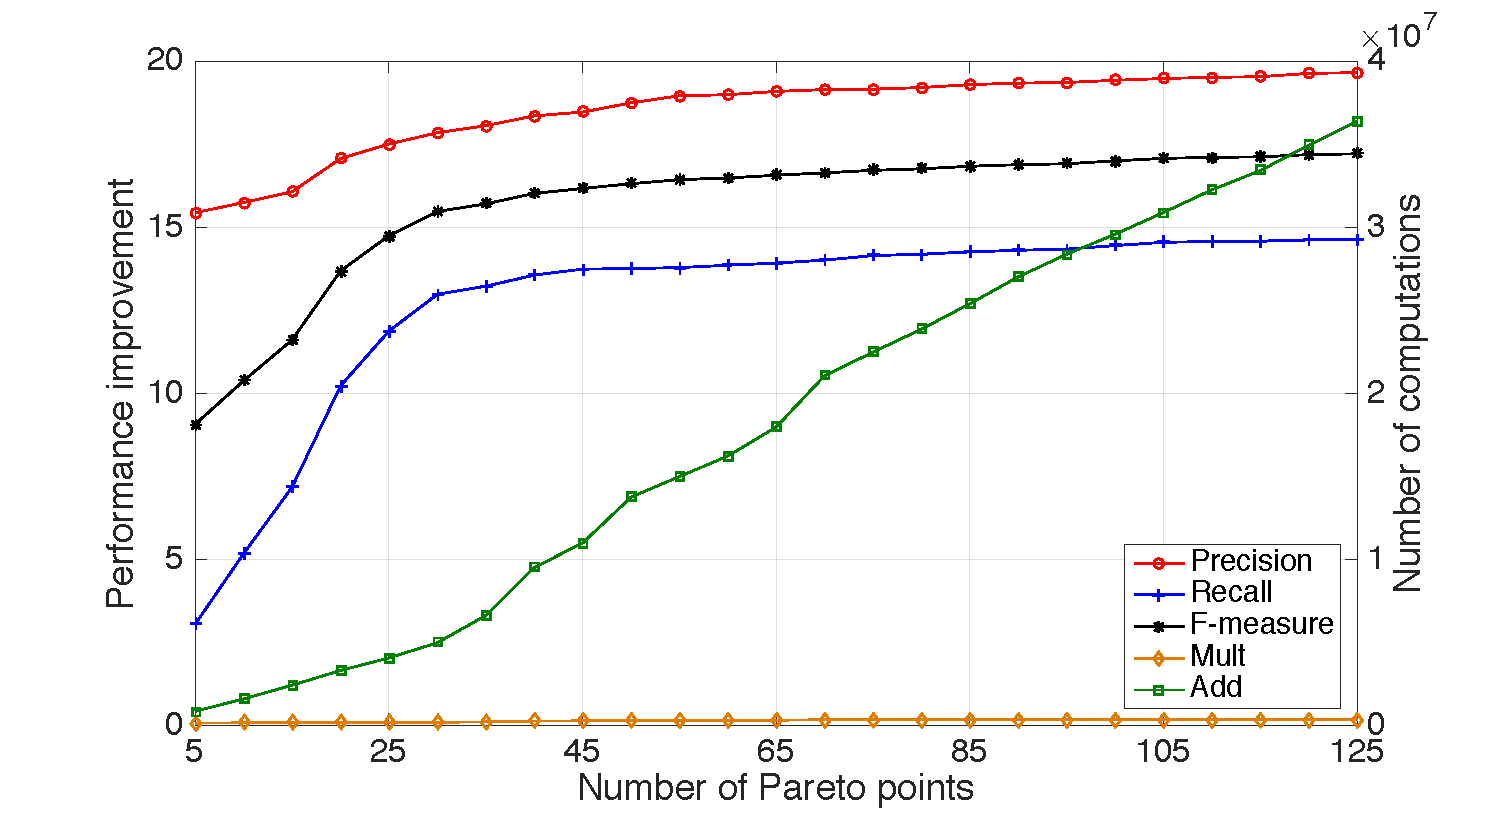
\includegraphics[width=0.8\textwidth]{./chapters/chapter5/images/R1_cph_L.pdf}}
%  \vspace{1.5cm}
  \centerline{(a) REDD 1}\medskip
\end{minipage}
\hfill
\begin{minipage}[b]{1\linewidth}
  \centering
  \centerline{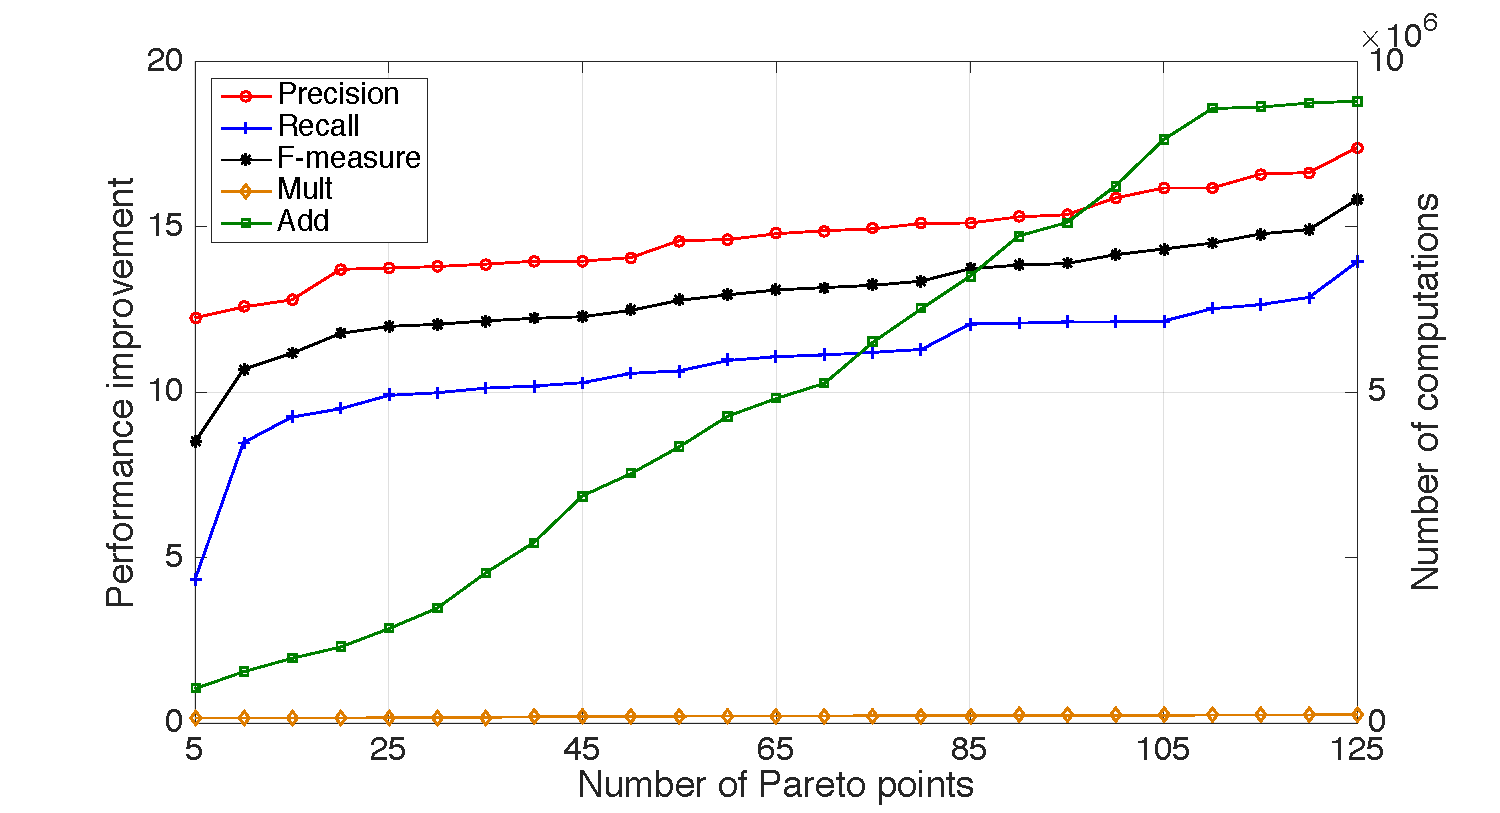
\includegraphics[width=0.8\textwidth]{./chapters/chapter5/images/R2_cph_L.pdf}}
%  \vspace{1.5cm}
  \centerline{(a) REDD 2}\medskip
\end{minipage}
\caption{Effect of the number of Pareto points on the performance and complexity of the CPH algorithm.}
\label{fig:SR9}
%
\end{figure}

\begin{figure}[htb]
\begin{minipage}[b]{1\linewidth}
  \centering
  \centerline{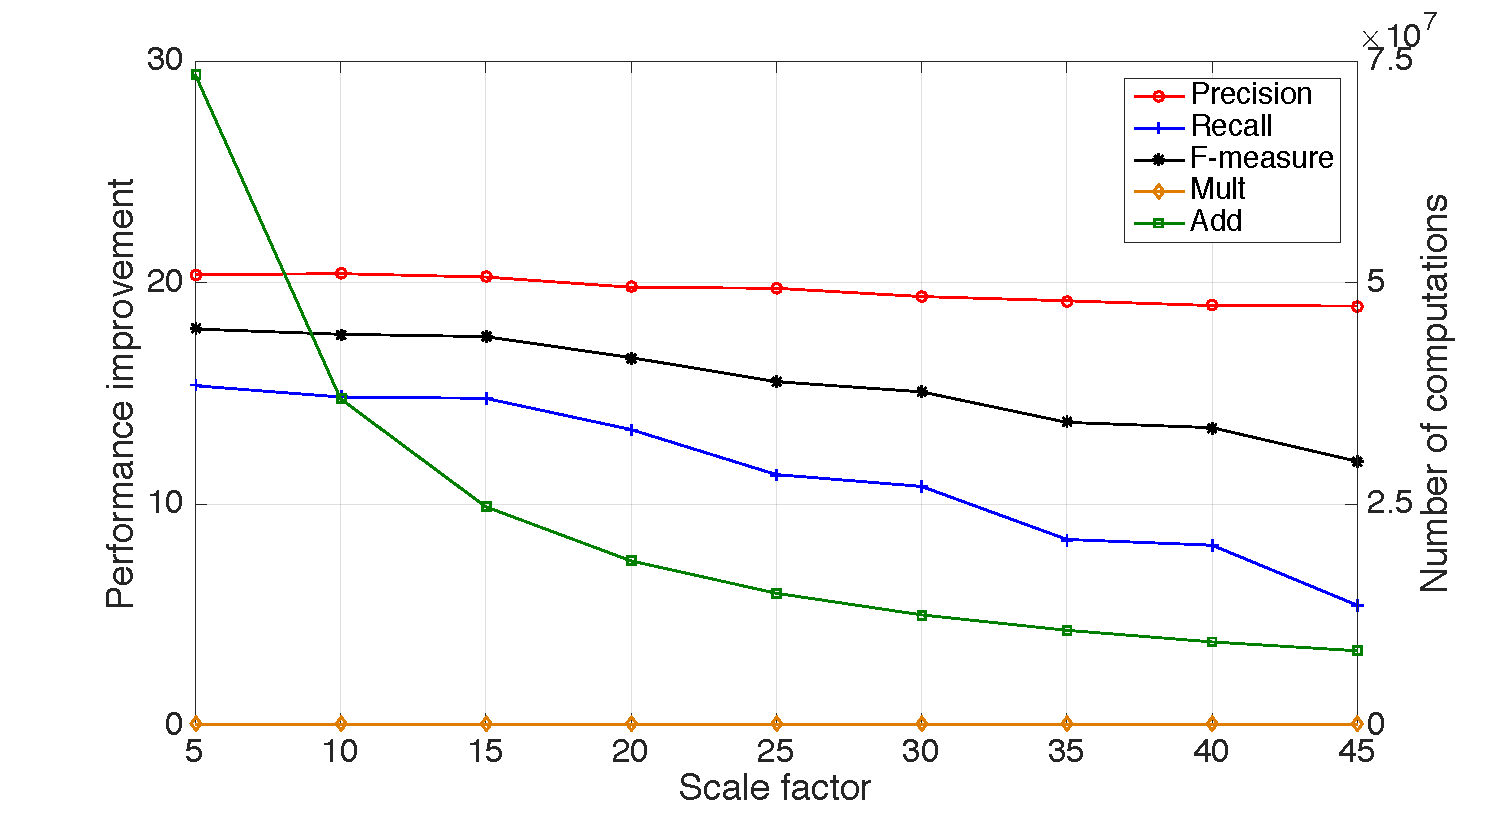
\includegraphics[width=0.8\textwidth]{./chapters/chapter5/images/R1_scale.pdf}}
%  \vspace{1.5cm}
  \centerline{(a) REDD 1}\medskip
\end{minipage}
\hfill
\begin{minipage}[b]{1\linewidth}
  \centering
  \centerline{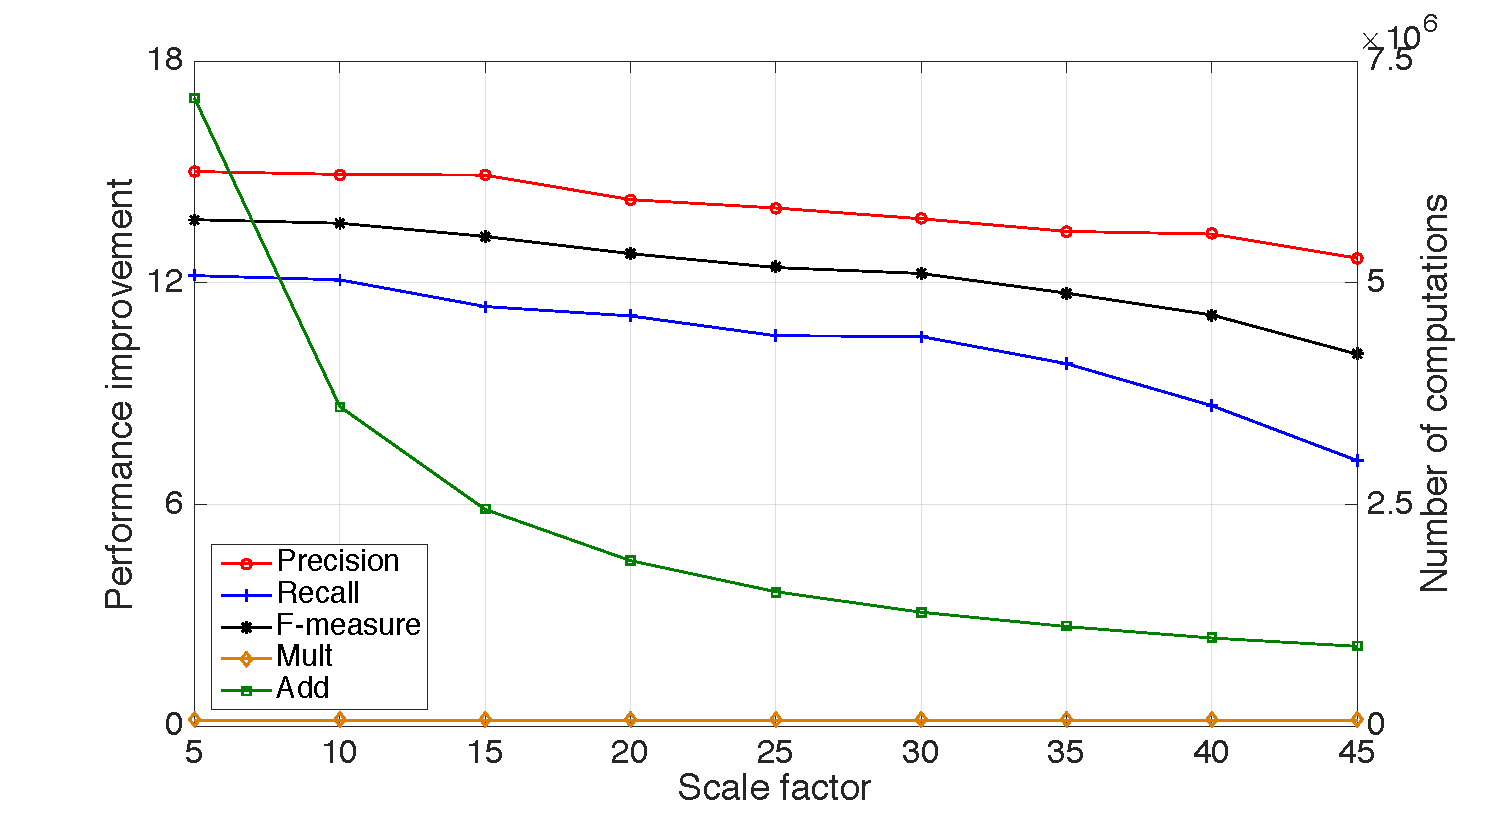
\includegraphics[width=0.8\textwidth]{./chapters/chapter5/images/R2_scale.pdf}}
%  \vspace{1.5cm}
  \centerline{(b) REDD 2}\medskip
\end{minipage}
\caption{Effect of the scale factor on the performance and complexity of the DP algorithm.}
\label{fig:SR10}
%
\end{figure}

Similar to CPH method, the DP algorithm also needs a large amount of computations. The principle of DP is based on the construction of profit tables. Therefore, the computational complexity depends on the size of each table, correlating to the number of devices, the aggregate power and the number of computations in each cell, decided by the number of states of current device. As a consequence, the complexity reduction effort can be executed by decreasing the number of columns with a scale factor $\delta$, e.g. $w_{ij} = w_{ij}/\delta,i=1,\ldots,N,j=1,\ldots,m_i$, $R = R/\delta$. If possible, the best choice of $\delta$ is the common divisor of $R$ and $w_{ij}$. However, this condition is unrealistic and the effect of the rounding down operation makes the performance decrease, as shown in Figure~\ref{fig:SR10}.
In the DP algorithm, the construction of the profit tables is only based on the addition. This is the reason why the scale factor only affects the number of additions and does not change the number of multiplications, as illustrated in Figure~\ref{fig:SR10}(a). The results with REDD~1 in case with two monitored devices show a decrease of the number of additions from $7.35\times 10^7$ to $8.43\times 10^6$ when increasing the scale factor from 5 to 45. The performance of the algorithm also attenuates respectively by the precision gain from 24.5$\%$ to 19$\%$ and the recall gain from 15.2$\%$ to 5.5$\%$. Meanwhile, Figure~\ref{fig:SR10}(b) presents the attenuation of the performance gain from 15$\%$ to 12.7$\%$ of precision and from 12.2$\%$ to 7.2$\%$ of recall when the value of $\delta$ increases from 5 to 45 in REDD~2. This tuning also allows to significantly decrease the number of computations. Concretely, the additions reduce from $7.08\times 10^6$ to $9\times 10^5$.

Different from the algorithms in the knapsack approach, both ED and DTW are less complex. Apparently, the computational complexity of the ED algorithm depends on the number of patterns in the library. If each of the $N$ devices has $m$ patterns, the device identification procedure needs to browse $Nm$ times to find the minimum distance. Meanwhile, because taking all power values in a pattern into account, besides the number of patterns in the library, the complexity of the DTW algorithm is also decided by the length of each one. If each pattern has an average length of $l$, the accumulated distance calculation has a complexity of $l^2$, which makes the DTW become an $Nml^2$-complex algorithm. 
Despite less complexity, both ED and DTW algorithms are not suitable for the real-time application. They need to detect the falling edge before pairing with the rising one and identifying the corresponding device during this period. On the contrary, when applied to real-time energy disaggregation, the complexity of the CPH and DP one is compatible for implementation in an NILM system, since the algorithm is applied on the main system measuring the global energy consumption.

\section{Conclusions}
In this chapter, we introduce a new load monitoring system, which uses a WSN to detect and provide the operating probability of some devices to help the NILM algorithms in improving their performance. This system is called sensor-aided non-intrusive load monitoring (SmartSense). Although deploying a sensors network, SmartSense is less intrusive than other intrusive load monitoring systems such as ViridiScope~\cite{Kim09Ubicomp}, because only a subset of all devices is selected to attach with the sensors and the identification is still based on an NILM algorithm.
The operation probability is used as a feature and combined with the traditional features of NILM by a regularization parameter to create a new one. In this chapter, two approaches are proposed:
\begin{itemize}
\item Knapsack approach: the $l1$-norm minimization problem in \cite{Hart92} is modeled as a knapsack problem and solved by two proposed algorithms including compositional Pareto-algebraic heuristic, which is based on a recursive relation, and dynamic programming, based the the construction of profit tables.
\item Edge detector approach: an edge detector is applied to detect the rising edge and falling edge of an activation on the aggregate power signal and to compare them with the existing ones in the library. The rising edge and falling edge can be directly used as a feature (as in edge detection algorithm) or combined with other active power values between them (as in dynamic time warping algorithm).
\end{itemize}

By simulating all four proposed algorithms with four dataset including UK-DALE~5, REDD~1, REDD~2 and our Athemium data, the performance of the load detection can be significantly improved with some monitored devices in comparison with traditional NILM systems. To obtain a good improvement, the devices selected to be monitored need to satisfy some criteria. In the knapsack approach, selected devices are the one with high using rate and confusion on the power demand with other devices. Meanwhile, the edge detector approach needs to monitor the devices more frequently switched on/off and ambiguous with the others on the edges height.
As a consequence, only several devices in home or building are selected, satisfying these requirements and allowing to significantly improve the overall performance when monitored. The others are less effective and need to be ignored when deploying the monitoring sensor network to reduce the cost. 

Besides, comparing the performance of the proposed approaches shows that the CPH and DP algorithms outperform the ED and DTW ones with more than two monitored devices in each dataset, although in normal NILM system, they are less effective. This result comes from the fact that the performance of the ED and DTW algorithms also depends on the edge detector capacity.

However, the algorithms of the knapsack approach show a high complexity presented by the large amount of multiplications and additions. To reduce the computational complexity, we can drive some parameters such as the number of Pareto points retained after each iteration in CPH or the scale factor in DP. Nevertheless, it also causes the attenuation of the performance. 

